\documentclass[10pt]{article}
\usepackage{amsmath, amssymb, amsfonts} % برای فرمول‌نویسی
\usepackage{breqn} % برای فرمول‌نویسی
\usepackage{amsthm}% برای اضافه کردن محیط proof
\usepackage{subfigure} % اضافه کردن شکل های زیر شکل ها
\usepackage{setspace} % تعیین فاصله بین خطوط
\usepackage{graphicx} % اضافه کردن عکس
\usepackage{multicol} % حروف چینی چند ستونه
\usepackage[margin=1in]{geometry} % تغییر دادن حاشیه دور
\usepackage{fancyvrb}
\usepackage{tcolorbox}
\usepackage{float}

\graphicspath{{./pics/}}

\usepackage{xepersian}

\settextfont{XB Yas} % برای ست کردن فونت متن
\setdigitfont{XB Zar} % برای ست کردن فونت اعداد

\setcounter{secnumdepth}{4} % Set Sections' Depth
\setcounter{tocdepth}{4}% Set Table Of Content's Depth

\title{پروژه درس سیستم‌های مخابراتی}
\author{نام و نام‌ خانوادگی : امیرحسین یاری
	\\ \\
	شماره دانشجویی : ۹۸۱۰۹۷۱۸ 	\\ \\
	تاریخ : ۲۰ بهمن ۱۴۰۰}
\date{}
\doublespacing

\begin{document}
	
	\maketitle
	\pagebreak
	\tableofcontents
	\newpage
	\section{توضیجات اولیه}
	کد‌های هر بخش در فولدر 
	\lr{Codes}
	قرار دارد و نتایج شبیه سازی در 
	\lr{img}
	قرار دارد.
	همچنین حروف چینی با استفاده از 
	\LaTeX
	بوده و فایل
	\lr{tex}
	مربوط به آن در فولدر 
	\lr{Tex}
	قرار دارد.
	
	\section{پیاده سازی بلوک ها به صورت مجزا}
	توابع مربوطه در فولدر 
	\lr{Codes}
	قرار داد.
	\subsection{\lr{Divide, Combine}}
	تابع 
	\lr{Divide}
	به این شکل نوشته شده که نمونه های فرد و زوج سیگنال را جدا میکند که یکی در میان است و نزدیک ترین حالت به سیستم
	\lr{Real-time}
	است.
	همچنین تابع
	\lr{Combine}
	معکوس ان سیستم است و دو ورودی را یکی در میان با هم ترکیب میکند تا دنباله خروجی را بسازد.
	
	
	\subsection{\lr{PulseShaping}}
	در این بخش تابع 
	\lr{PulseShaping}
	به این شکل نوشته شده است که به ازای یک در دنباله ورودی شکل موج مربوطه به یک را در خروجی میدهد و همینطور برای صفر که در نهایت منجر به خروجی با طول ضرب طول های دو دنباله ورودی و شکل یک میشود. 
	
	
	\subsection{\lr{AnalogMod}}
	این تابع تنها با ضرب ورودی اول در کسینوس و ضرب دومی در سینوس خروجی
	\lr{xc}
	را میدهد.
	
	\subsection{\lr{Channel}}
	این تابع با استفاده از فیلتر 
	\lr{bandpass}
	نوشته شده است که پارامتر
	\lr{steepness}
	تابع که میزان تیز بودن فیلتر است برای بخش سوم قسمت سه
	\lr{0.8}
	گرفته شده اما در مابقی حالات
	\lr{0.98}
	است.
	
	\subsection{\lr{AnalogDemod}}
	این تابع ابتدا ورودی اول را در کسینوس و دومی را در سینوس ضرب میکند و در نهایت از یک فیلتر
	\lr{lowpass}
	عبور میدهد تا به خروجی ها برسد.
	
	
	
	\subsection{\lr{MatchedFilt}}
	در این بخش نیز ابتدا پاسخ ضربه هر شکل را که معکوس شده ان است با ورودی کانولوشن میگیریم و سپس با برسی بزرگ تر بودن کدام نتیجه صفر یا یک بودن بیت خروجی را تخمین میزنیم. 
	
	
	\newpage
	\section{انتقال دنباله تصادفی صفر و یک}
	کد‌ مربوط به این سوال در 
	\lr{Q3.m}
	قرار داد.
	\subsection{\lr{PAM}}
	سیگنال های صفر و یک به شکل دنباله ای از یک و منفی یک به طول ده میلی ثانیه است که در نمودار های زیر مشخص است.

	\subsubsection{\lr{no Noise}}
	 فرایند ارسال شبیه سازی شده و خروجی هر بلوک در ادامه به ترتیب اورده شده است.
	 
	\begin{figure}[h]
		\centering
		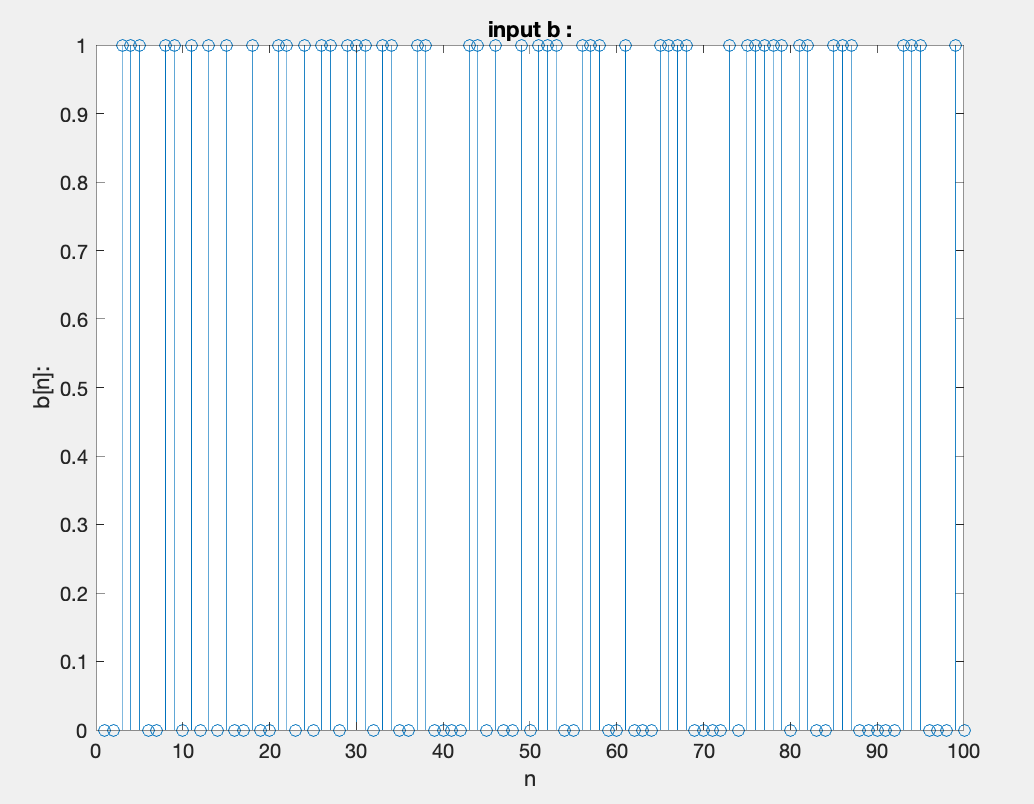
\includegraphics[width=0.5\linewidth]{../img/3.1.1}
		\caption{پیام ورودی}
		\label{fig:3-1-1}
	\end{figure}

	\begin{figure}[h]
		\centering
		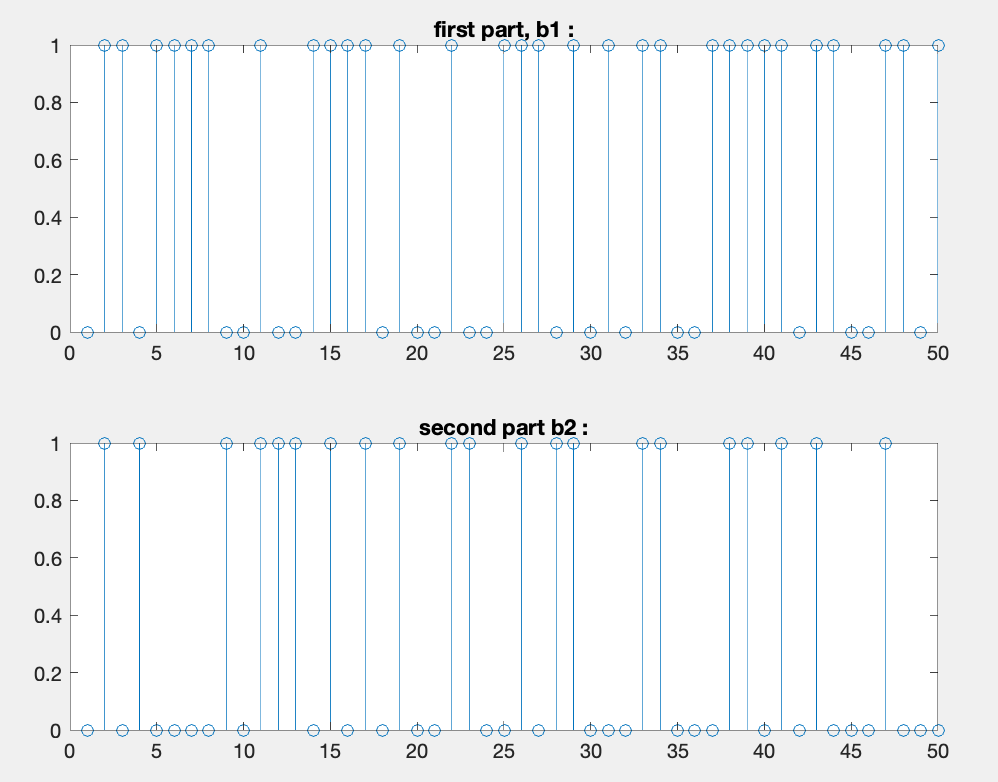
\includegraphics[width=0.5\linewidth]{../img/3.1.2}
		\caption{سیگنال های تقسیم شده}
		\label{fig:3-1-2}
	\end{figure}
	
	\begin{figure}[h]
		\centering
		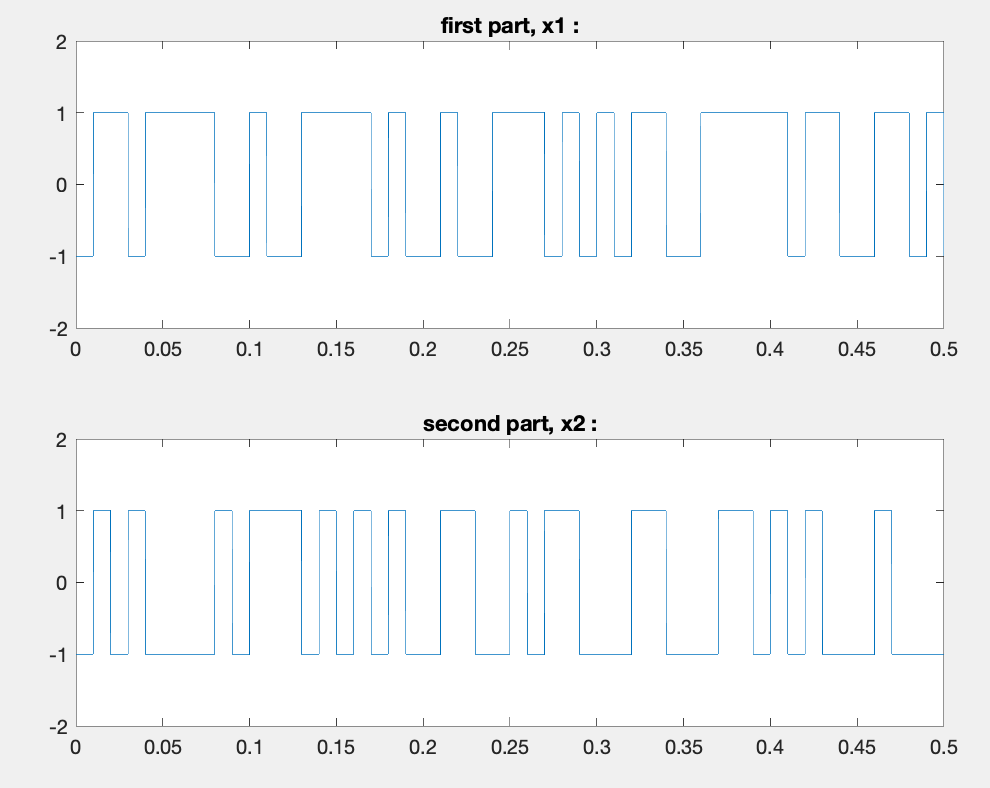
\includegraphics[width=0.5\linewidth]{../img/3.1.3}
		\caption{خروجی های
		 \lr{PalseShaping}}
		\label{fig:3-1-3}
	\end{figure}
	
	\begin{figure}[h]
		\centering
		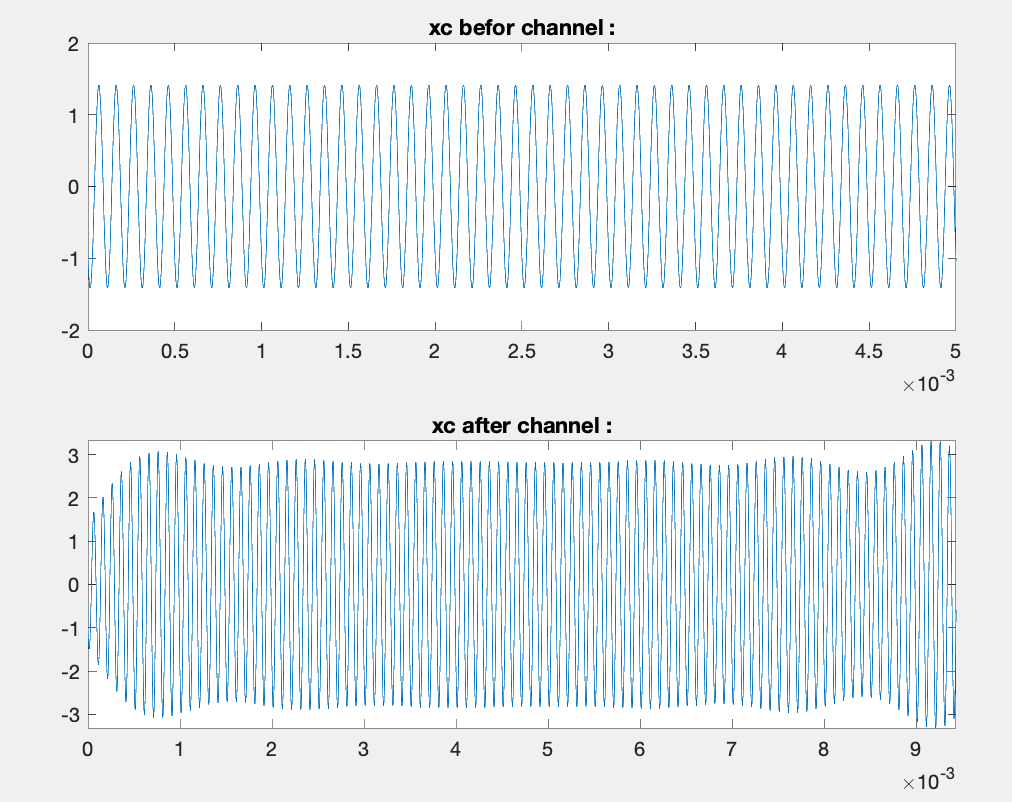
\includegraphics[width=0.5\linewidth]{../img/3.1.4}
		\caption{قبل و بعد از کانال}
		\label{fig:3-1-4}
	\end{figure}

	\newpage
	\begin{figure}[H]
		\centering
		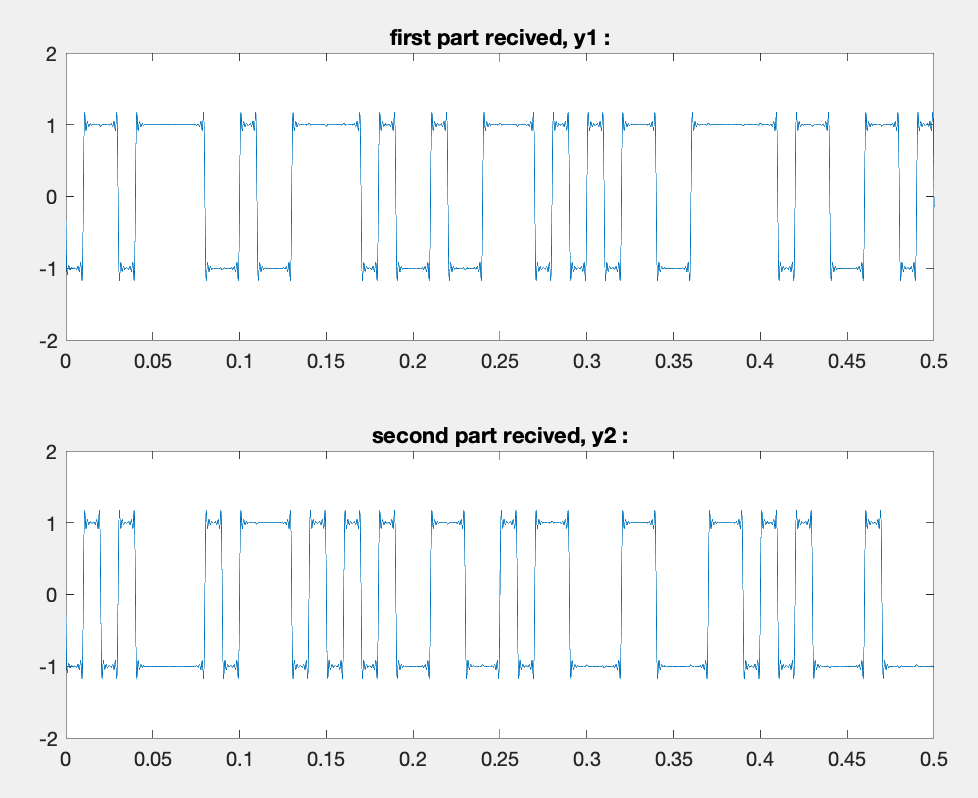
\includegraphics[width=0.5\linewidth]{../img/3.1.5}
		\caption{پس از بلوک 
		\lr{AnalogDemod}}
		\label{fig:3-1-5}
	\end{figure}


	\begin{figure}[h]
		\centering
		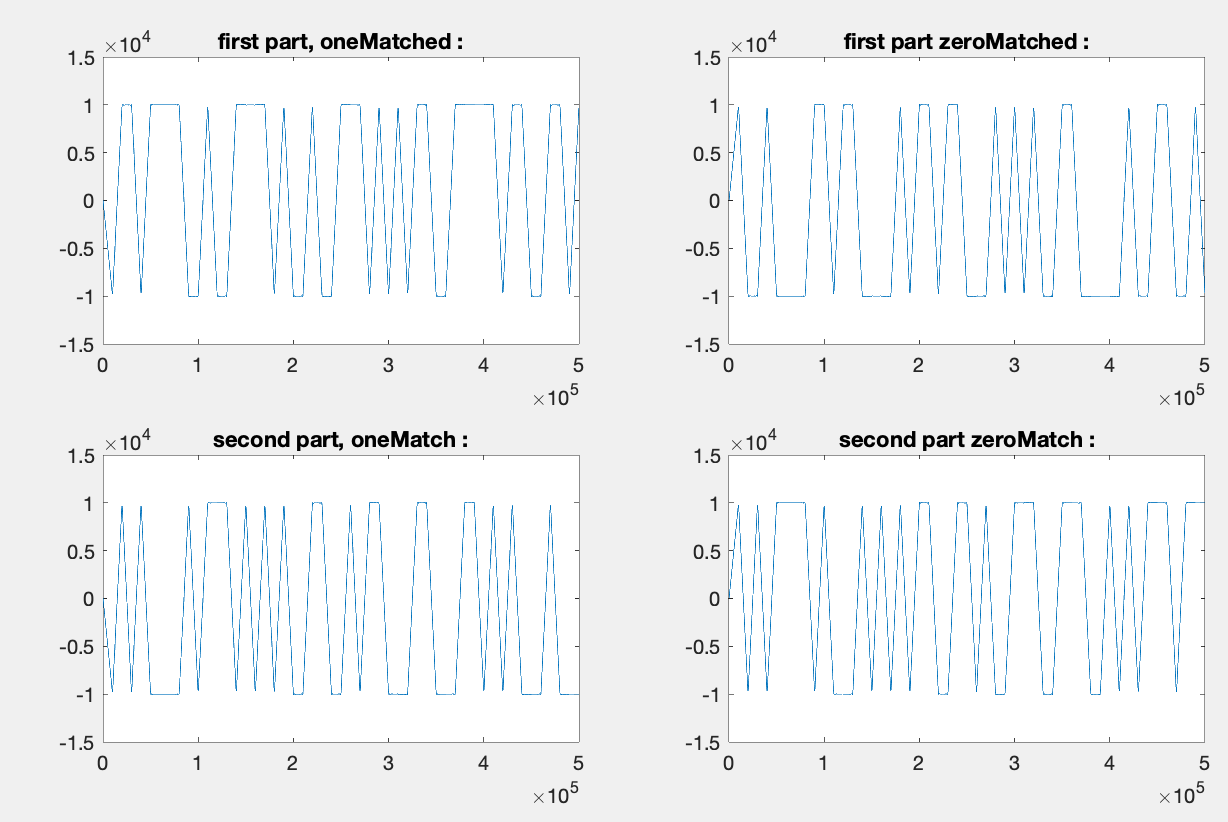
\includegraphics[width=0.6\linewidth]{../img/3.1.6}
		\caption{خروجی های کانولوشن بلوک 
		\lr{MatchedFilt}}
		\label{fig:3-1-6}
	\end{figure}

	\begin{figure}[h]
		\centering
		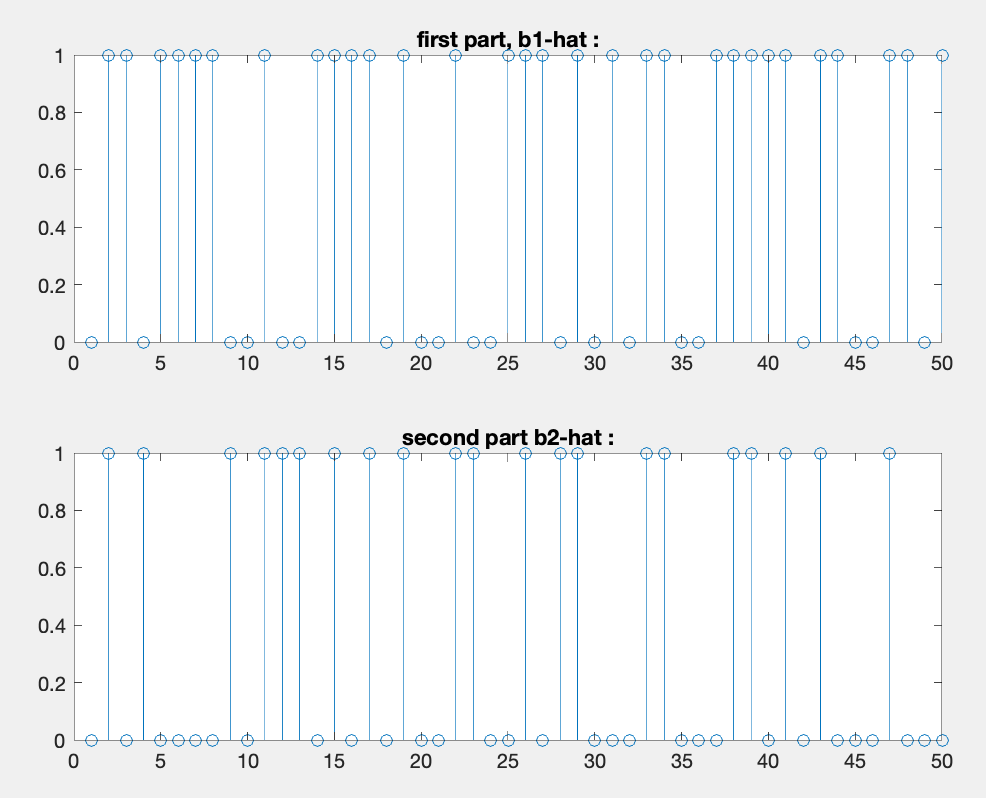
\includegraphics[width=0.5\linewidth]{../img/3.1.7}
		\caption{خروجی دنباله 
		\lr{MatchedFilt}}
		\label{fig:3-1-7}
	\end{figure}

	\begin{figure}[h]
		\centering
		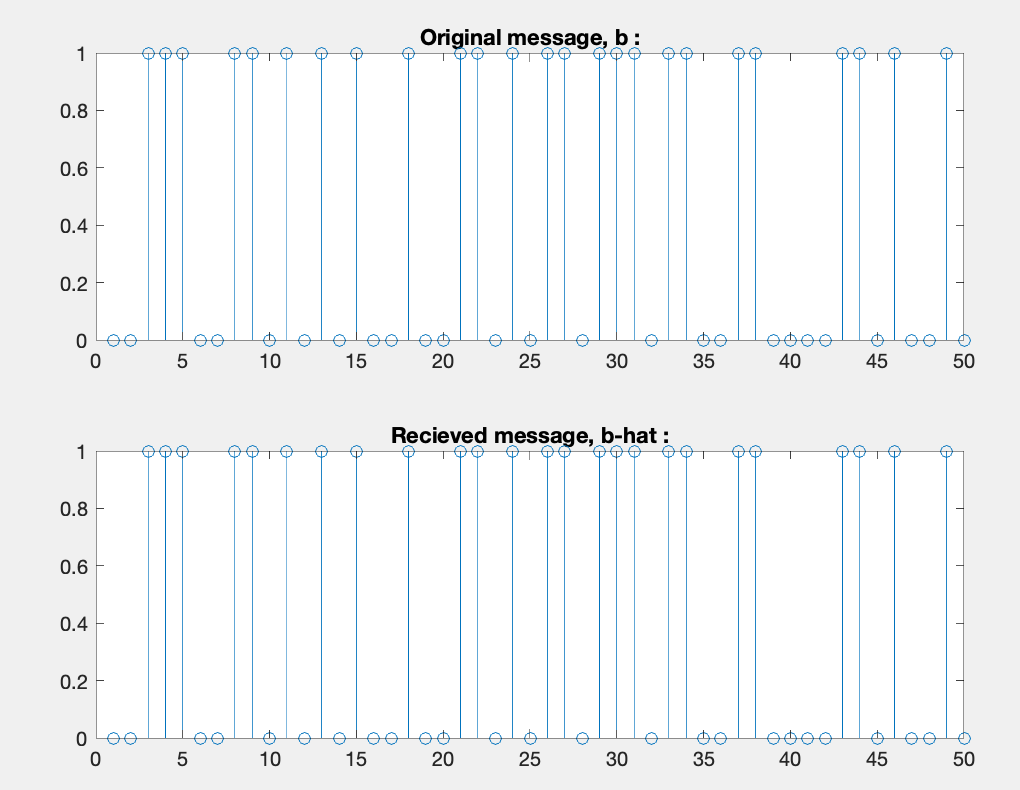
\includegraphics[width=0.7\linewidth]{../img/3.1.8}
		\caption{پیام دریافتی و فرستاده شده}
		\label{fig:3-1-8}
	\end{figure}
	
	
	
	\newpage
	\subsubsection{\lr{AWGN for PAM} }
	در این بخش واریانس خطا را افزایش میدهیم و میزان احتمال خطا نموداری مانند زیر خواهد داشت.
	\begin{figure}[H]
		\centering
		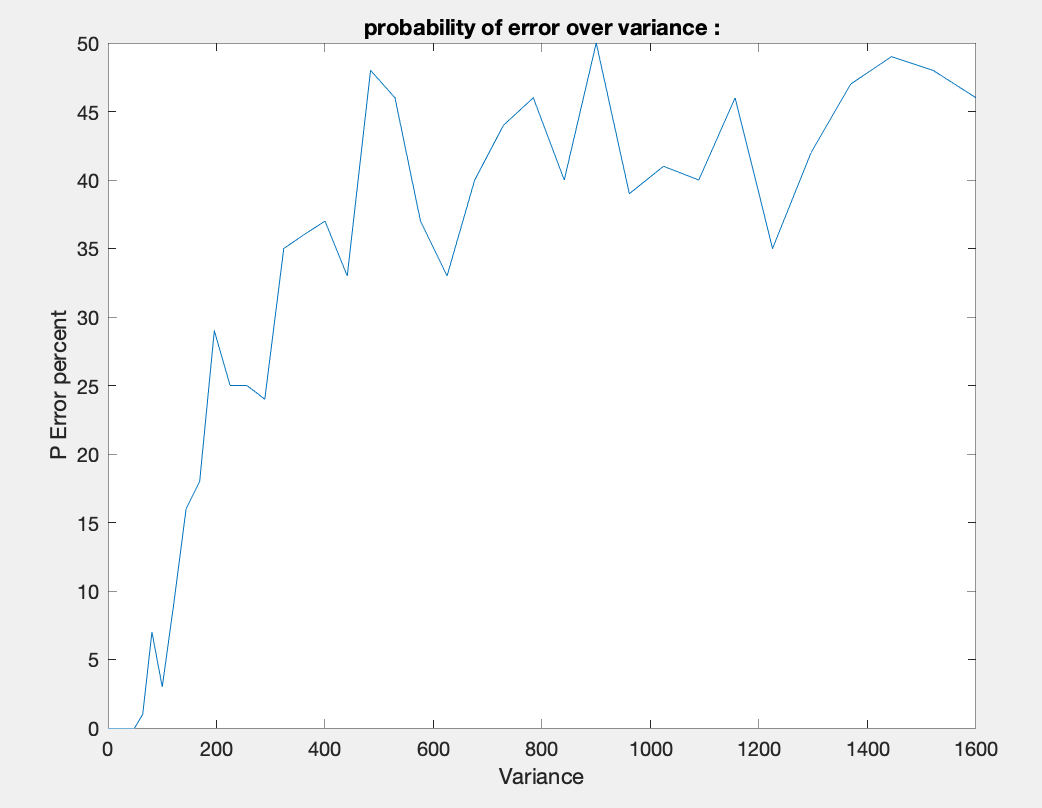
\includegraphics[width=0.6\linewidth]{../img/3.1.10}
		\caption{نمودار خطا بر حسب واریانس نویز}
		\label{fig:3-1-10}
	\end{figure}

\newpage
	همچنین نمودار در بازه بزرگ تر مانند زیر است که به احتمال پنجاه درصد میل میکند که به دلیل کاملا رندوم شدن خروجی با توجه به نویز زیاد است.
	\begin{figure}[H]
		\centering
		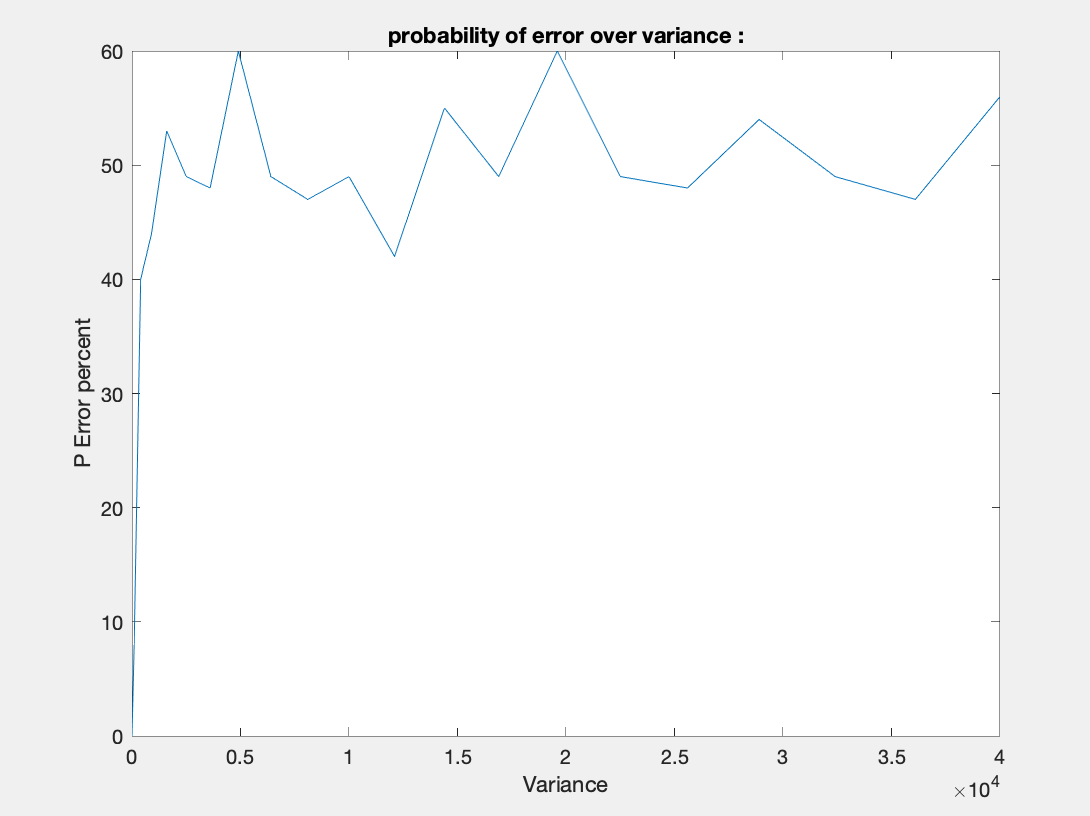
\includegraphics[width=0.6\linewidth]{../img/3.1.9}
		\caption{نمودار خطا بر حسب واریانس نویز در بازه بزرگ تر}
		\label{fig:3-1-9}
	\end{figure}
	
	\newpage
	\subsubsection{\lr{Scatter Plot}}
	در این بخش نمودار منظومه سیگنال به ازای شش واریانس مختلف مانند زیر رسم شده است که هر چه واریانس افزایش میابد فشردگی نقاط حول نقاط اصلی کم تر و کم تر میشود.
	\begin{figure}[H]
		\centering
		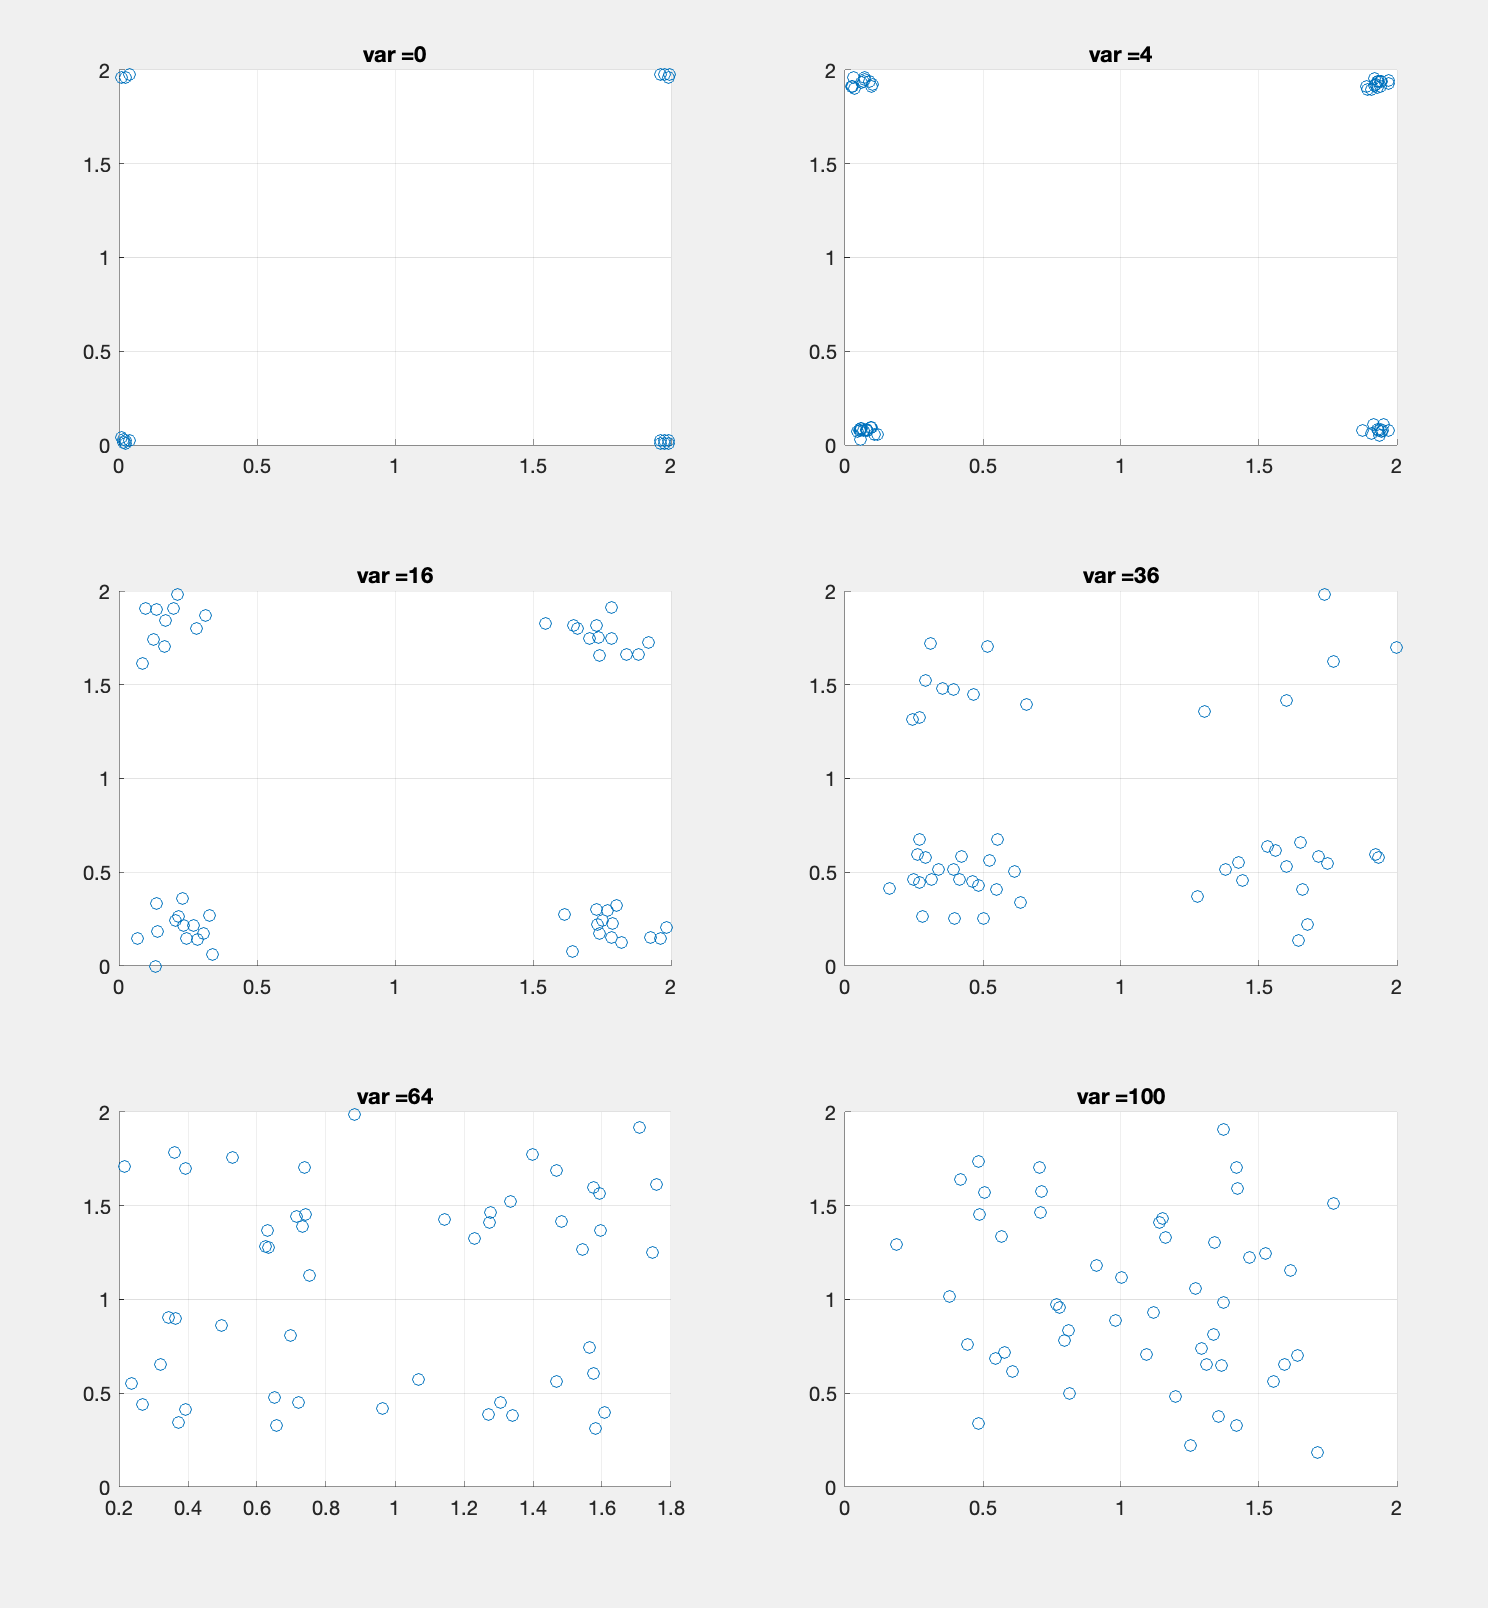
\includegraphics[width=0.8\linewidth]{../img/3.1.11}
		\caption{منظومه سیگنالی}
		\label{fig:3-1-11}
	\end{figure}



	\newpage
	\subsection{\lr{PSK}}
	سیگنال های صفر و یک به شکل سینوس و منفی سینوس با فرکانس پانصد هرتز استفاده شده است.
	
	\subsubsection{\lr{no Noise}}
	فرایند ارسال شبیه سازی شده و خروجی هر بلوک در ادامه به ترتیب اورده شده است.
	
	\begin{figure}[h]
		\centering
		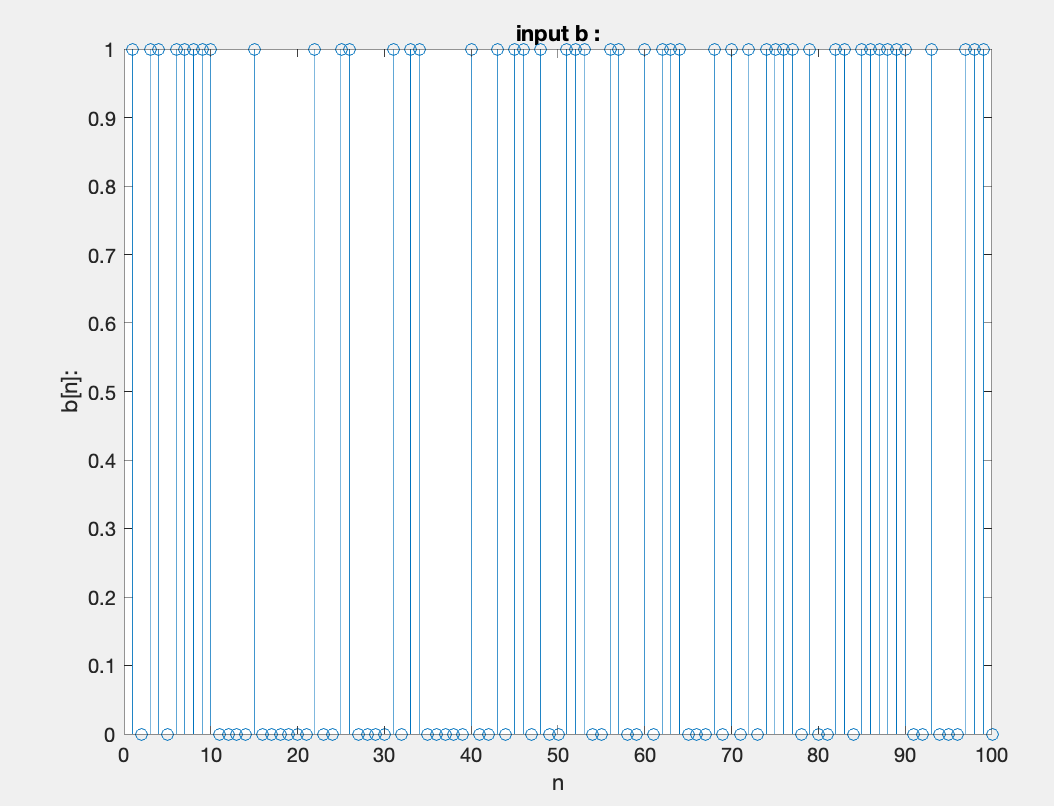
\includegraphics[width=0.5\linewidth]{../img/3.2.1}
		\caption{پیام ورودی}
		\label{fig:3-2-1}
	\end{figure}
	
	\begin{figure}[h]
		\centering
		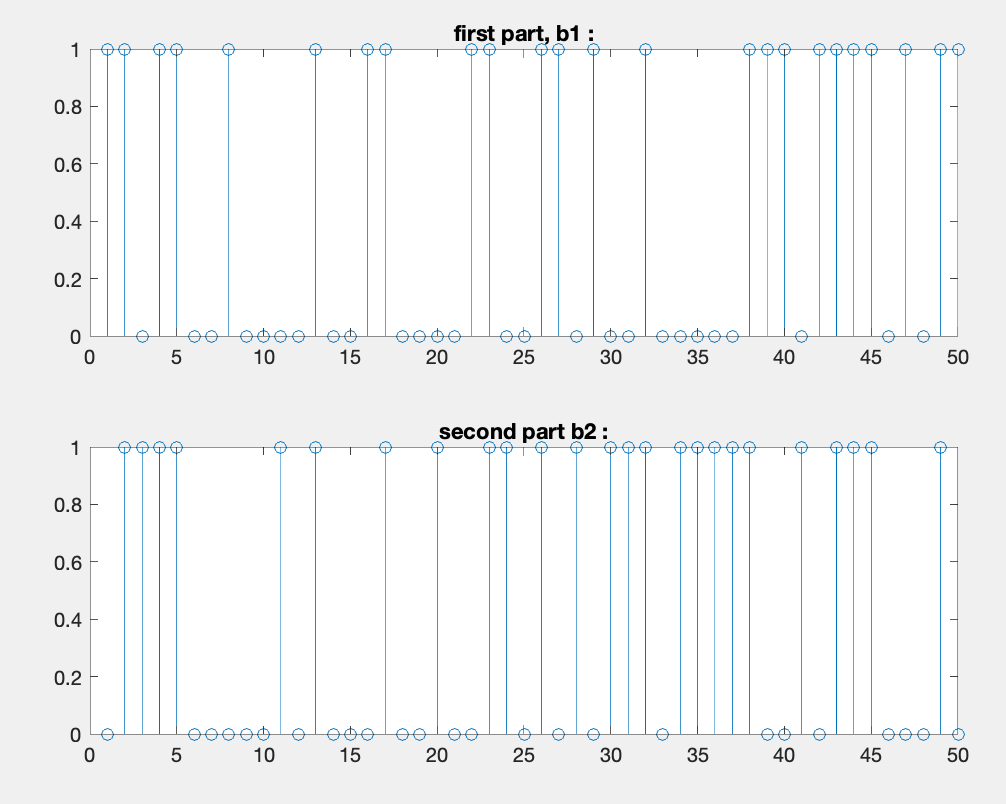
\includegraphics[width=0.5\linewidth]{../img/3.2.2}
		\caption{سیگنال های تقسیم شده}
		\label{fig:3-2-2}
	\end{figure}
	
	\begin{figure}[h]
		\centering
		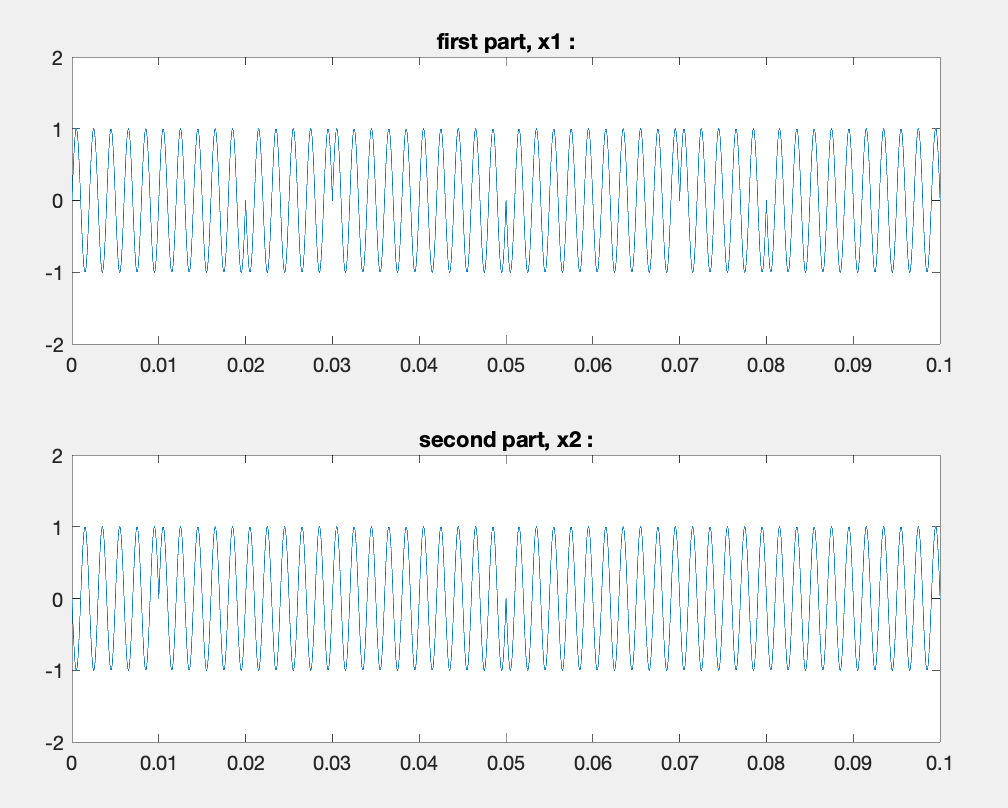
\includegraphics[width=0.5\linewidth]{../img/3.2.3}
		\caption{خروجی های
			\lr{PalseShaping}}
		\label{fig:3-2-3}
	\end{figure}
	
	\begin{figure}[h]
		\centering
		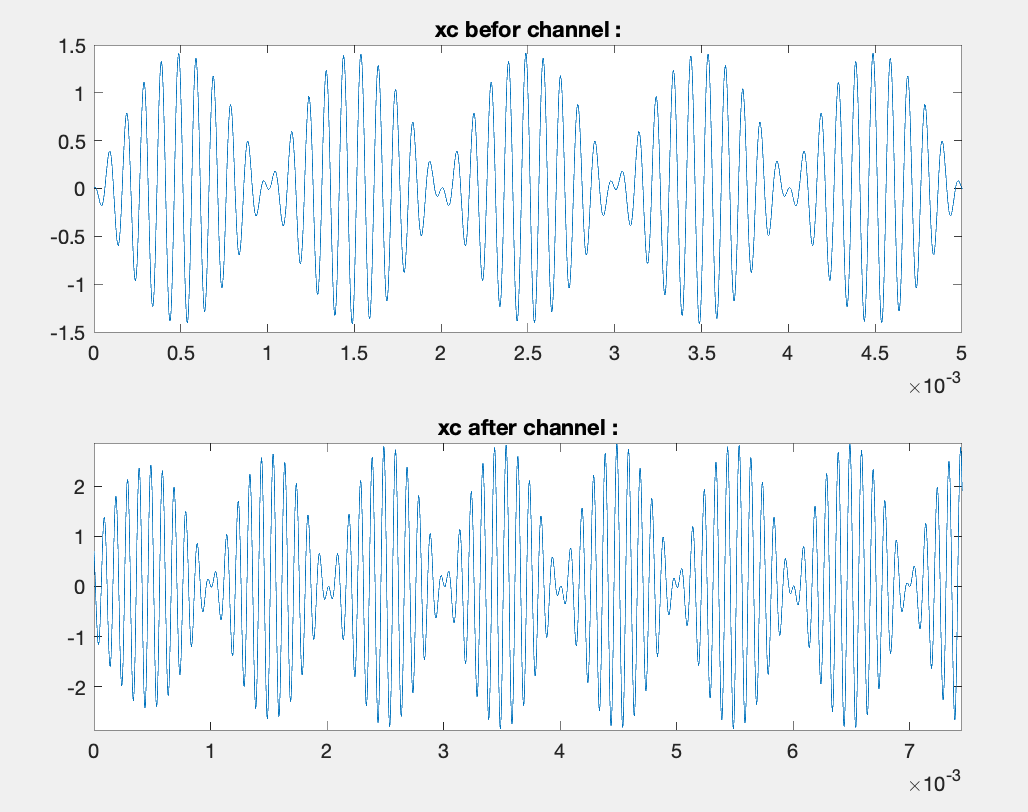
\includegraphics[width=0.5\linewidth]{../img/3.2.4}
		\caption{قبل و بعد از کانال}
		\label{fig:3-2-4}
	\end{figure}
	
	\newpage
	\begin{figure}[H]
		\centering
		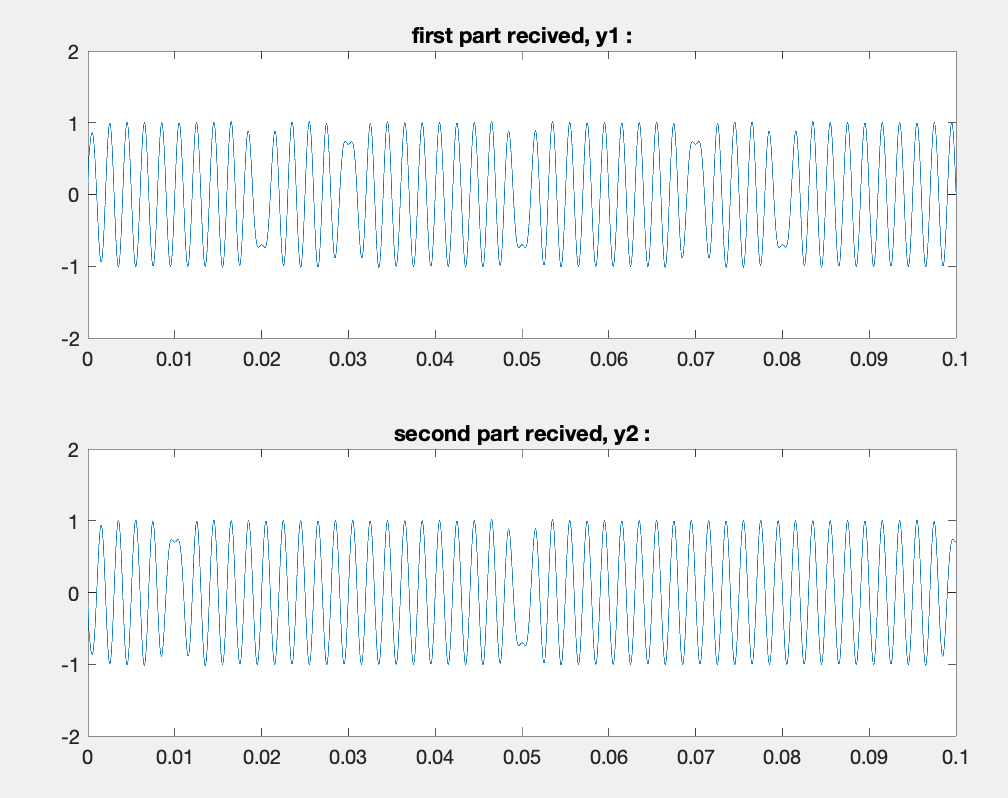
\includegraphics[width=0.5\linewidth]{../img/3.2.5}
		\caption{پس از بلوک 
			\lr{AnalogDemod}}
		\label{fig:3-2-5}
	\end{figure}
	
	
	\begin{figure}[h]
		\centering
		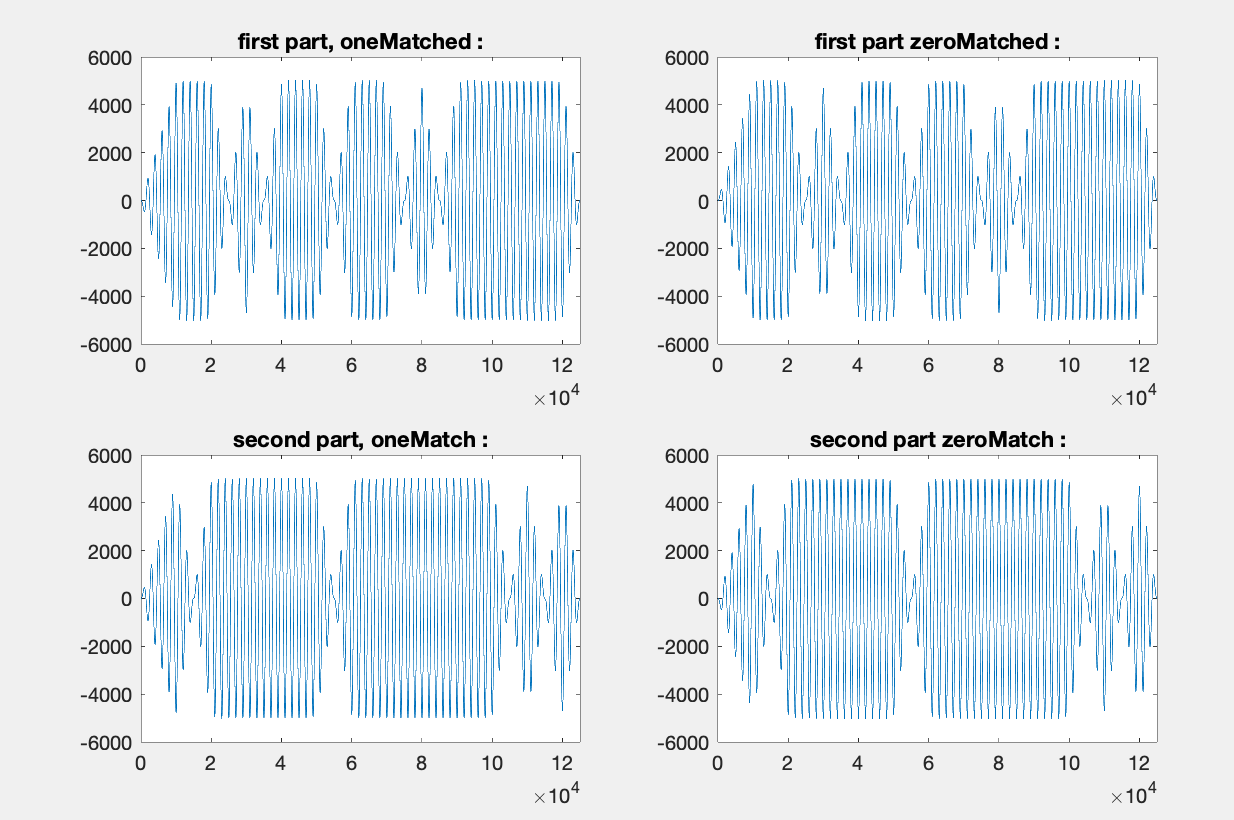
\includegraphics[width=0.6\linewidth]{../img/3.2.6}
		\caption{خروجی های کانولوشن بلوک 
			\lr{MatchedFilt}}
		\label{fig:3-2-6}
	\end{figure}
	
	\begin{figure}[h]
		\centering
		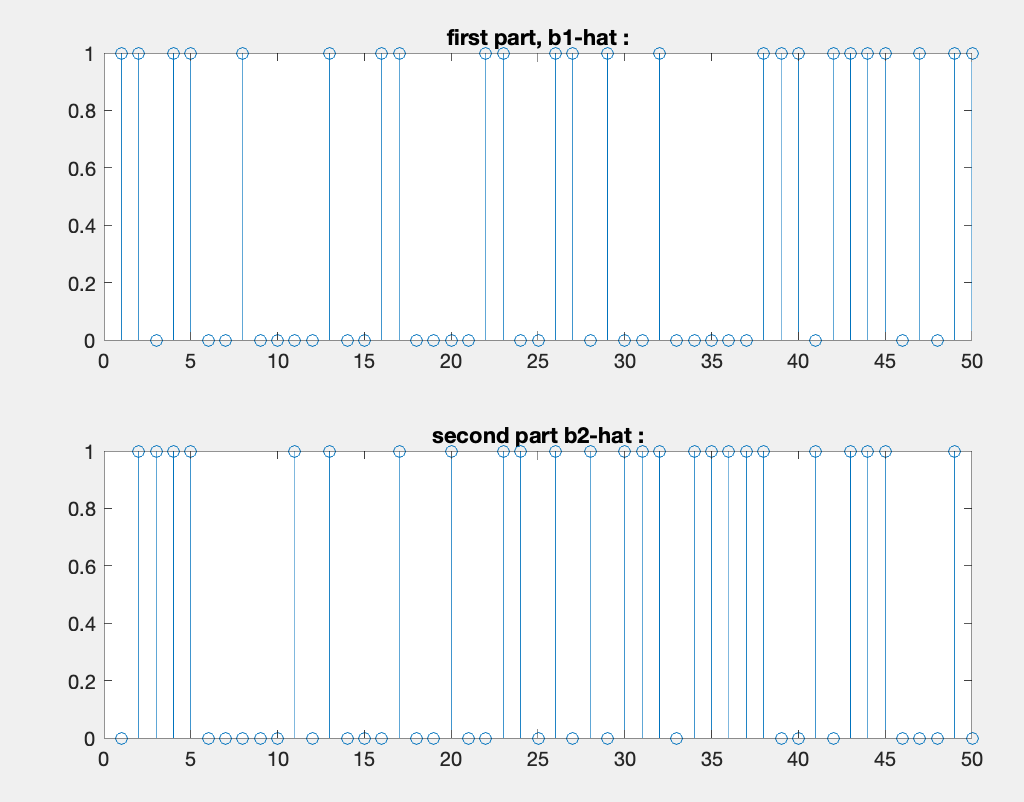
\includegraphics[width=0.5\linewidth]{../img/3.2.7}
		\caption{خروجی دنباله 
			\lr{MatchedFilt}}
		\label{fig:3-2-7}
	\end{figure}
	
	\begin{figure}[h]
		\centering
		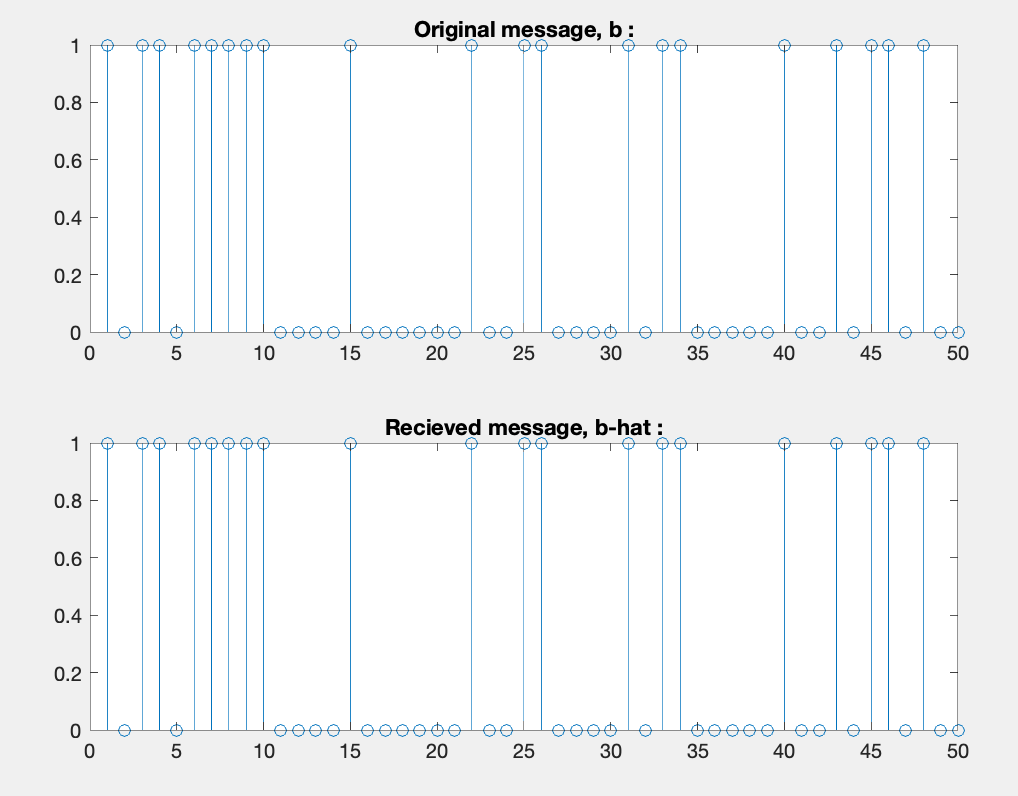
\includegraphics[width=0.7\linewidth]{../img/3.2.8}
		\caption{پیام دریافتی و فرستاده شده}
		\label{fig:3-2-8}
	\end{figure}
	
	
	
	\newpage
	\subsubsection{\lr{AWGN for PSK} }
	در این بخش واریانس خطا را افزایش میدهیم و میزان احتمال خطا نموداری مانند زیر خواهد داشت.
	\begin{figure}[H]
		\centering
		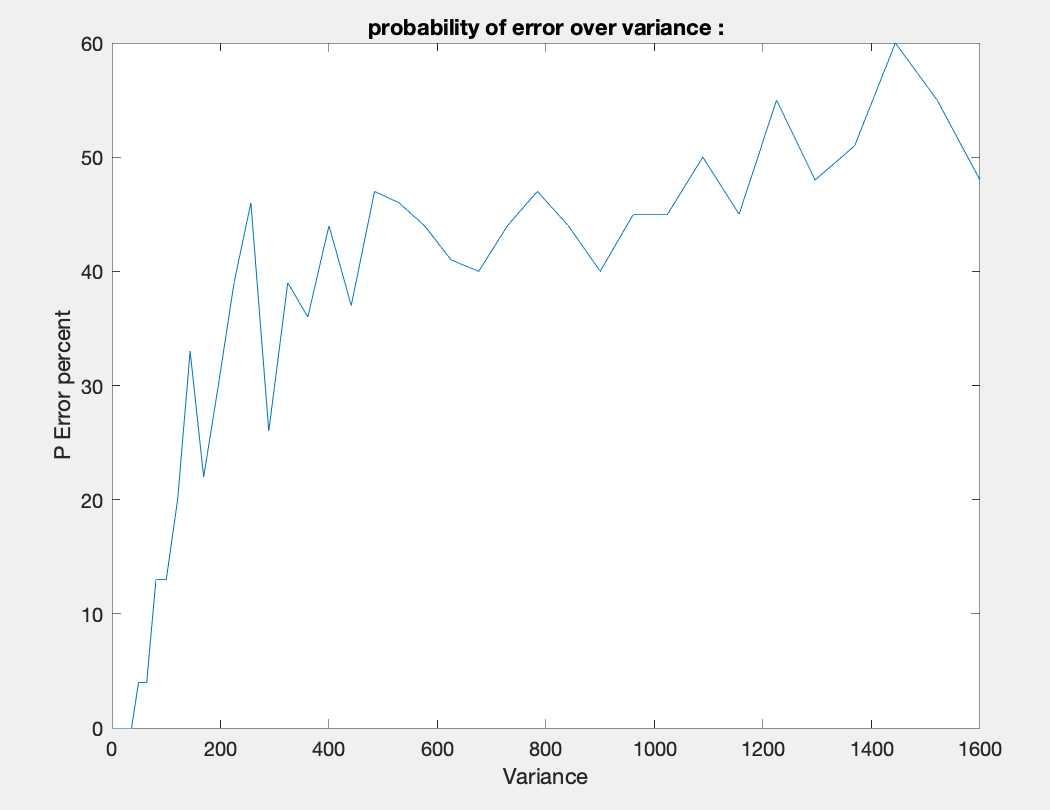
\includegraphics[width=0.6\linewidth]{../img/3.2.10}
		\caption{نمودار خطا بر حسب واریانس نویز}
		\label{fig:3-2-10}
	\end{figure}
	
	\newpage
	همچنین نمودار در بازه بزرگ تر مانند زیر است که به احتمال پنجاه درصد میل میکند که به دلیل کاملا رندوم شدن خروجی با توجه به نویز زیاد است.
	\begin{figure}[H]
		\centering
		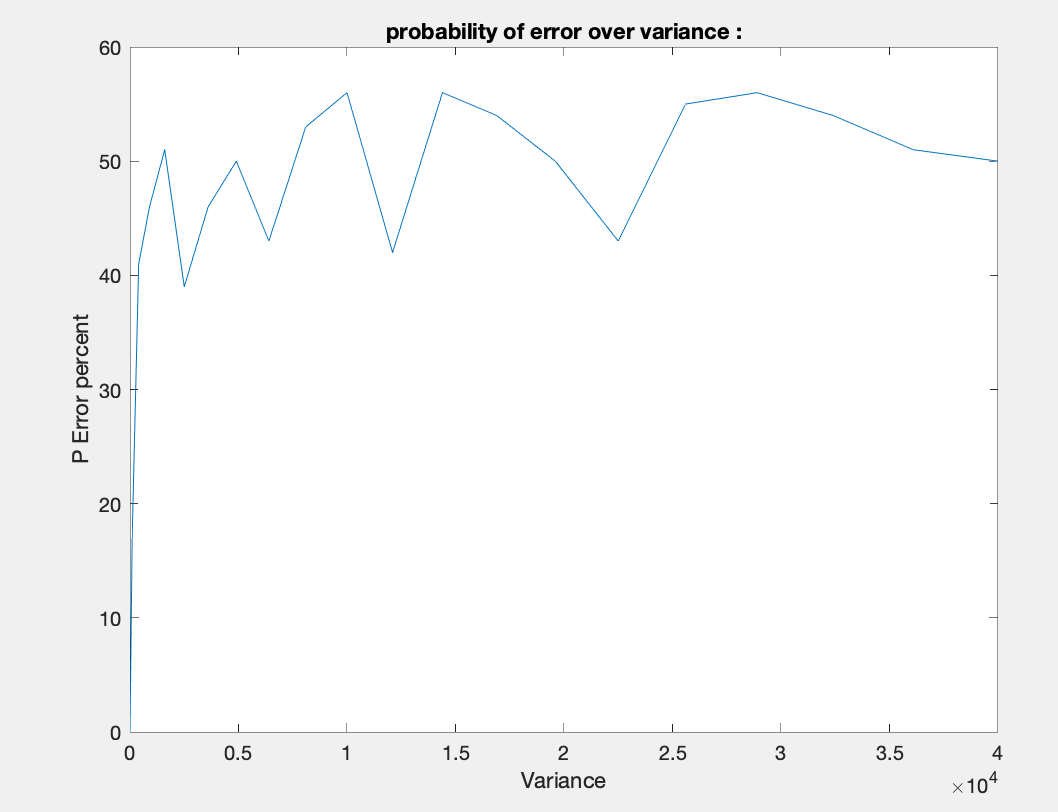
\includegraphics[width=0.6\linewidth]{../img/3.2.9}
		\caption{نمودار خطا بر حسب واریانس نویز در بازه بزرگ تر}
		\label{fig:3-2-9}
	\end{figure}
	
	\newpage
	\subsubsection{\lr{Scatter Plot}}
	در این بخش نمودار منظومه سیگنال به ازای شش واریانس مختلف مانند زیر رسم شده است که هر چه واریانس افزایش میابد فشردگی نقاط حول نقاط اصلی کم تر و کم تر میشود.
	\begin{figure}[H]
		\centering
		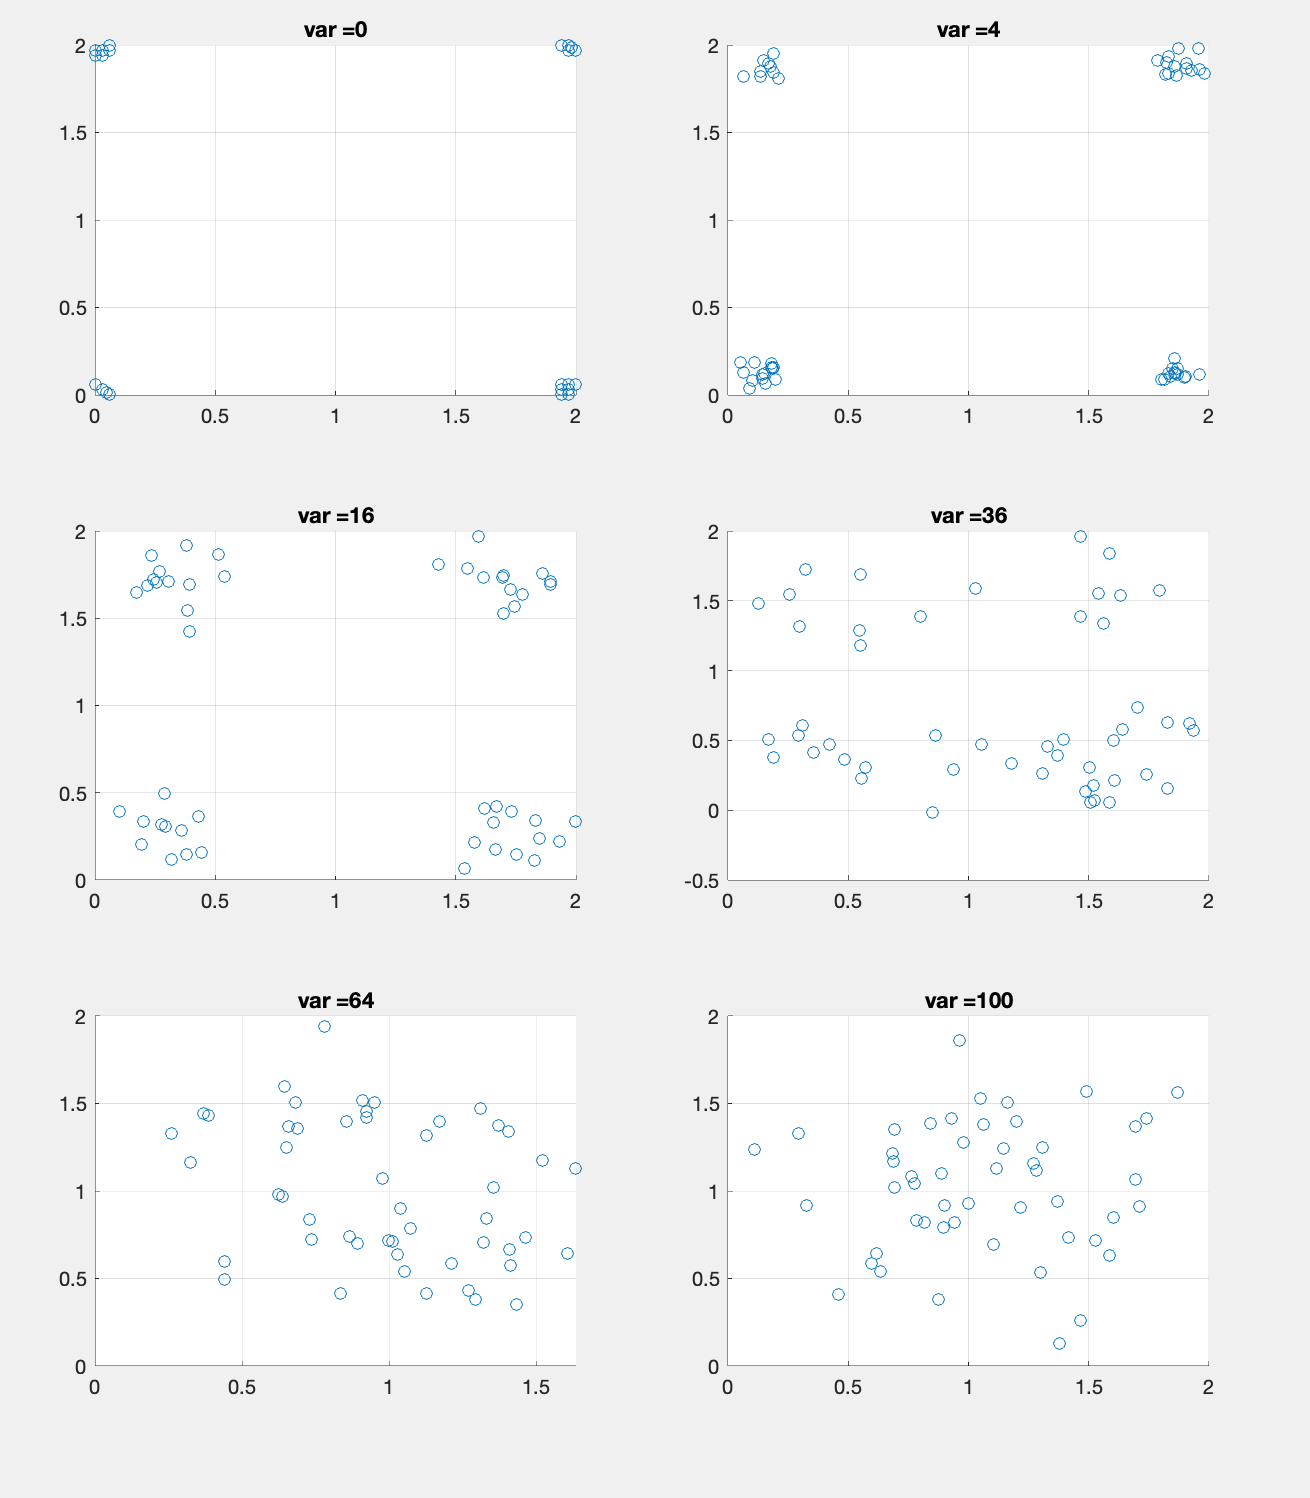
\includegraphics[width=0.8\linewidth]{../img/3.2.11}
		\caption{منظومه سیگنالی}
		\label{fig:3-2-11}
	\end{figure}



	\newpage
	\subsection{\lr{FSK}}
	سیگنال های صفر و یک به شکل سینوس با فرکانس یک کیلو نیم کیلو و سینوس با فرکانس یک کیلو هرتز استفاده شده است. که بر هم عمودند و یک سیگنالینگ متعامد میسازد.
	
	\subsubsection{\lr{no Noise}}
	فرایند ارسال شبیه سازی شده و خروجی هر بلوک در ادامه به ترتیب اورده شده است.
	
	\begin{figure}[h]
		\centering
		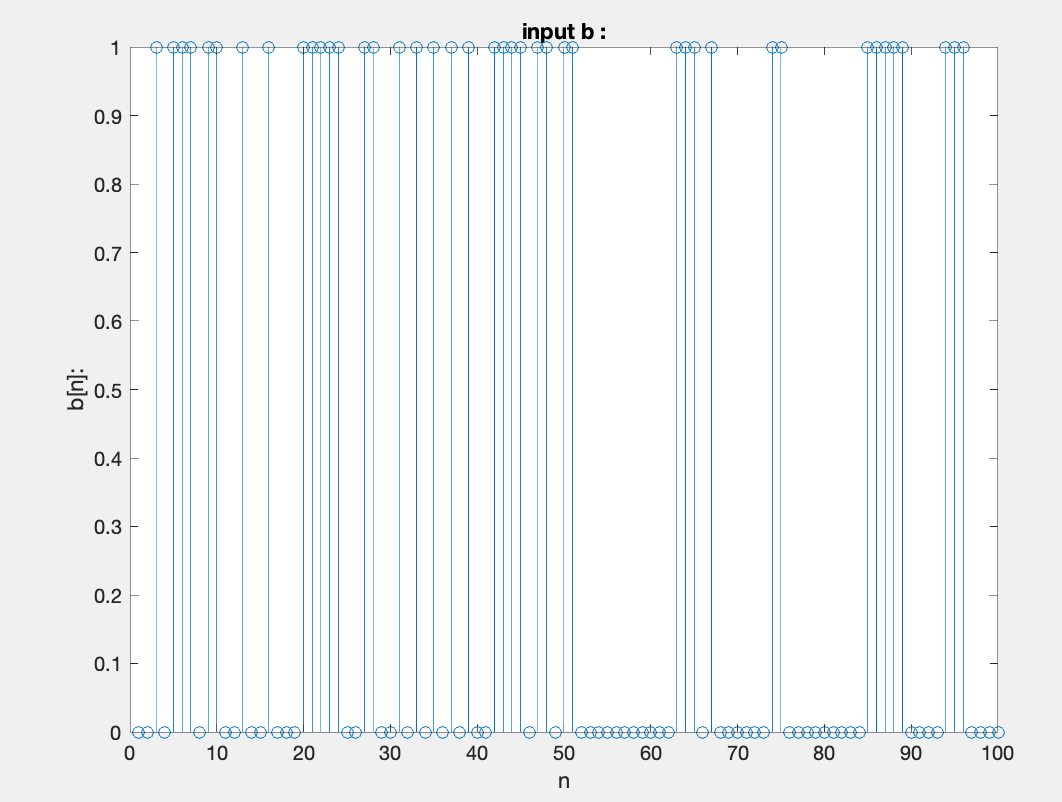
\includegraphics[width=0.5\linewidth]{../img/3.3.1}
		\caption{پیام ورودی}
		\label{fig:3-3-1}
	\end{figure}
	
	\begin{figure}[h]
		\centering
		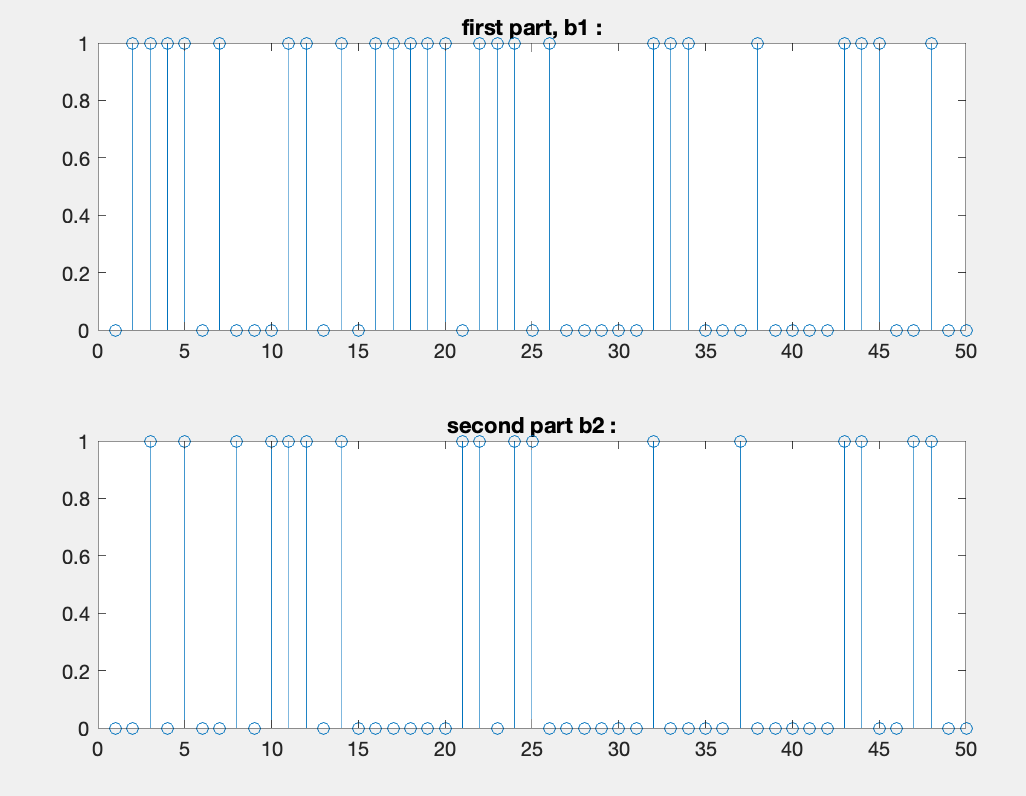
\includegraphics[width=0.5\linewidth]{../img/3.3.2}
		\caption{سیگنال های تقسیم شده}
		\label{fig:3-3-2}
	\end{figure}
	
	\begin{figure}[h]
		\centering
		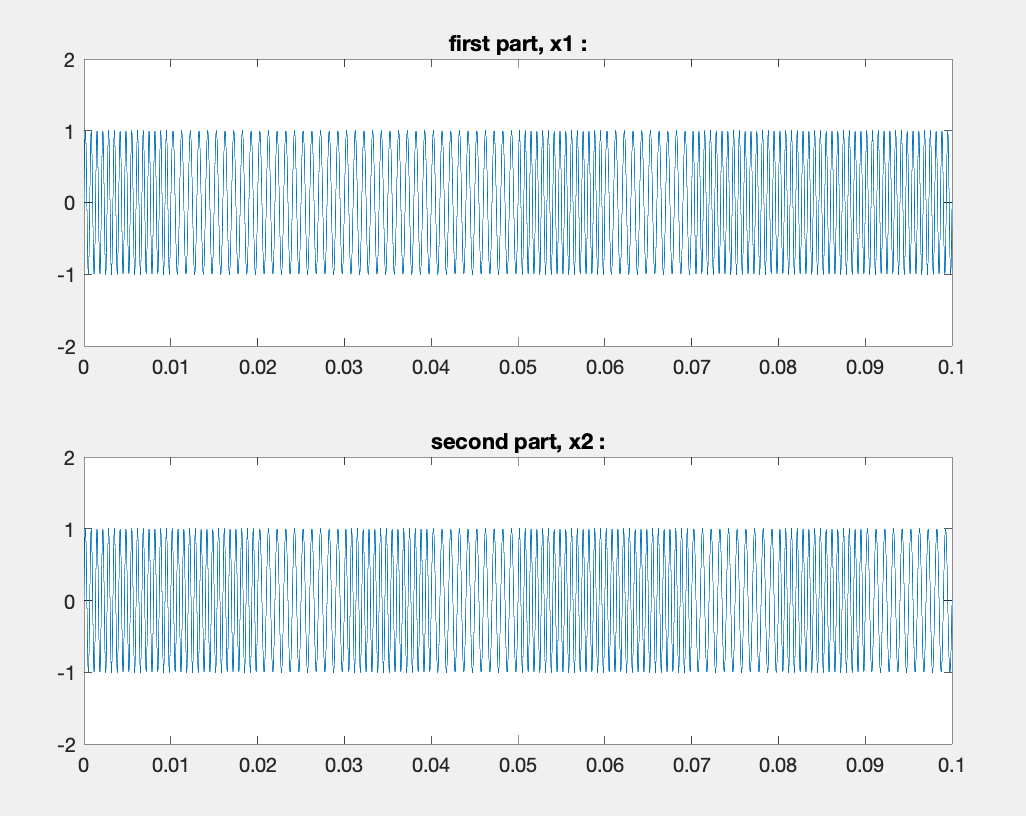
\includegraphics[width=0.5\linewidth]{../img/3.3.3}
		\caption{خروجی های
			\lr{PalseShaping}}
		\label{fig:3-3-3}
	\end{figure}
	
	\begin{figure}[h]
		\centering
		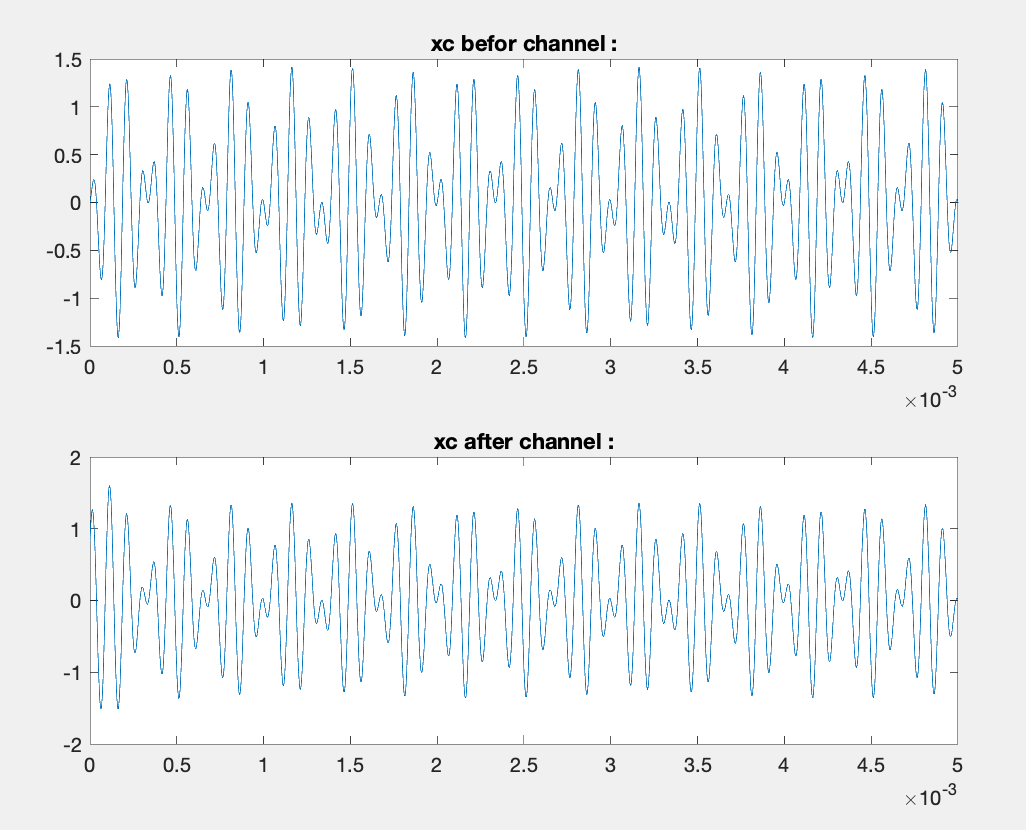
\includegraphics[width=0.5\linewidth]{../img/3.3.4}
		\caption{قبل و بعد از کانال}
		\label{fig:3-3-4}
	\end{figure}
	
	\newpage
	\begin{figure}[H]
		\centering
		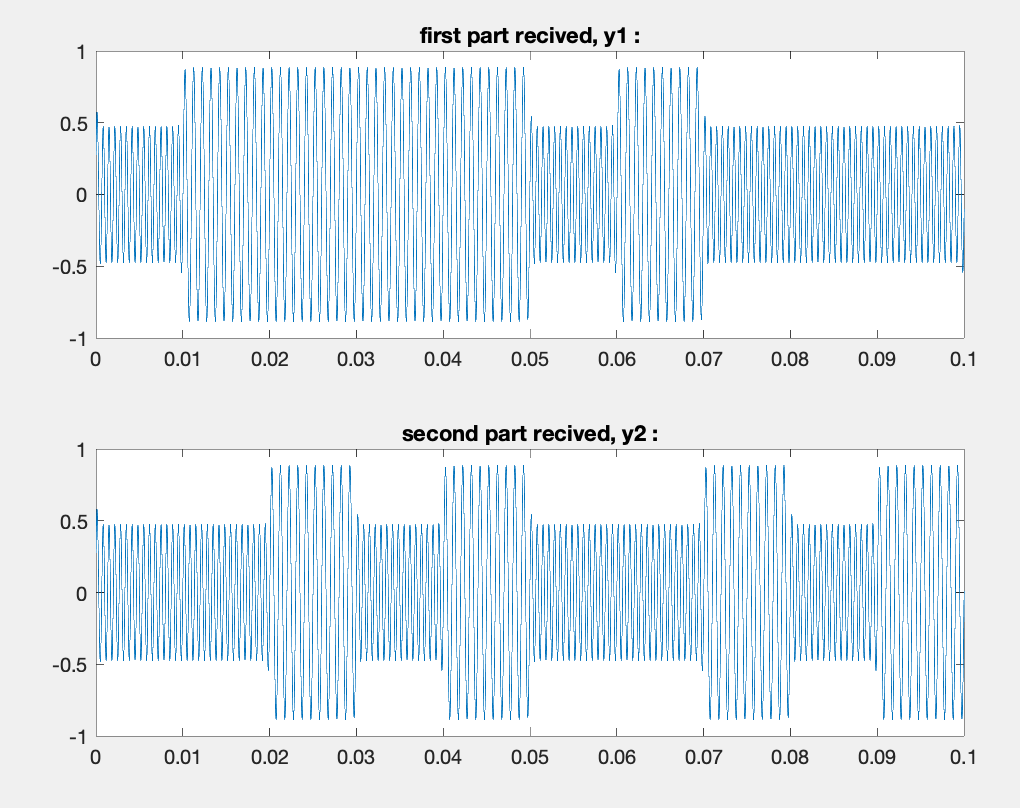
\includegraphics[width=0.5\linewidth]{../img/3.3.5}
		\caption{پس از بلوک 
			\lr{AnalogDemod}}
		\label{fig:3-3-5}
	\end{figure}
	
	
	\begin{figure}[h]
		\centering
		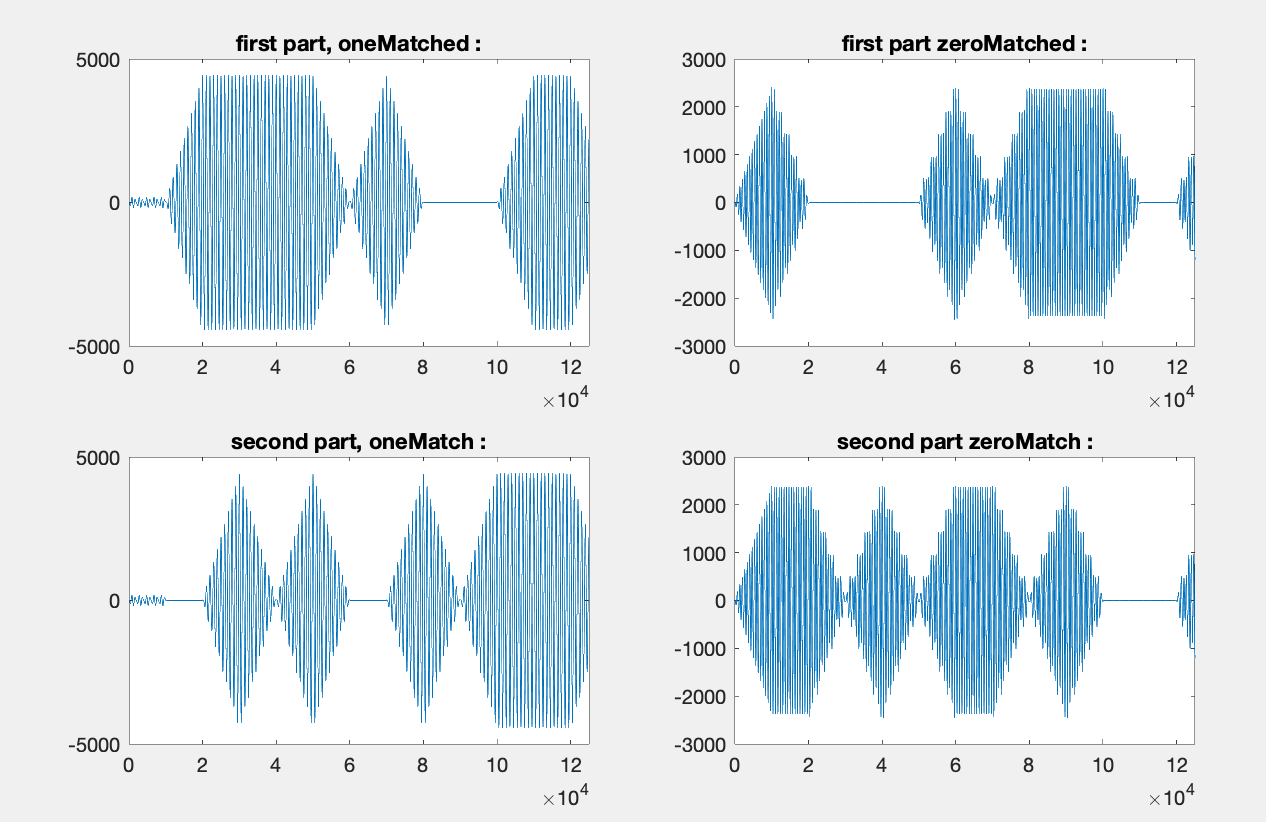
\includegraphics[width=0.6\linewidth]{../img/3.3.6}
		\caption{خروجی های کانولوشن بلوک 
			\lr{MatchedFilt}}
		\label{fig:3-3-6}
	\end{figure}
	
	\begin{figure}[h]
		\centering
		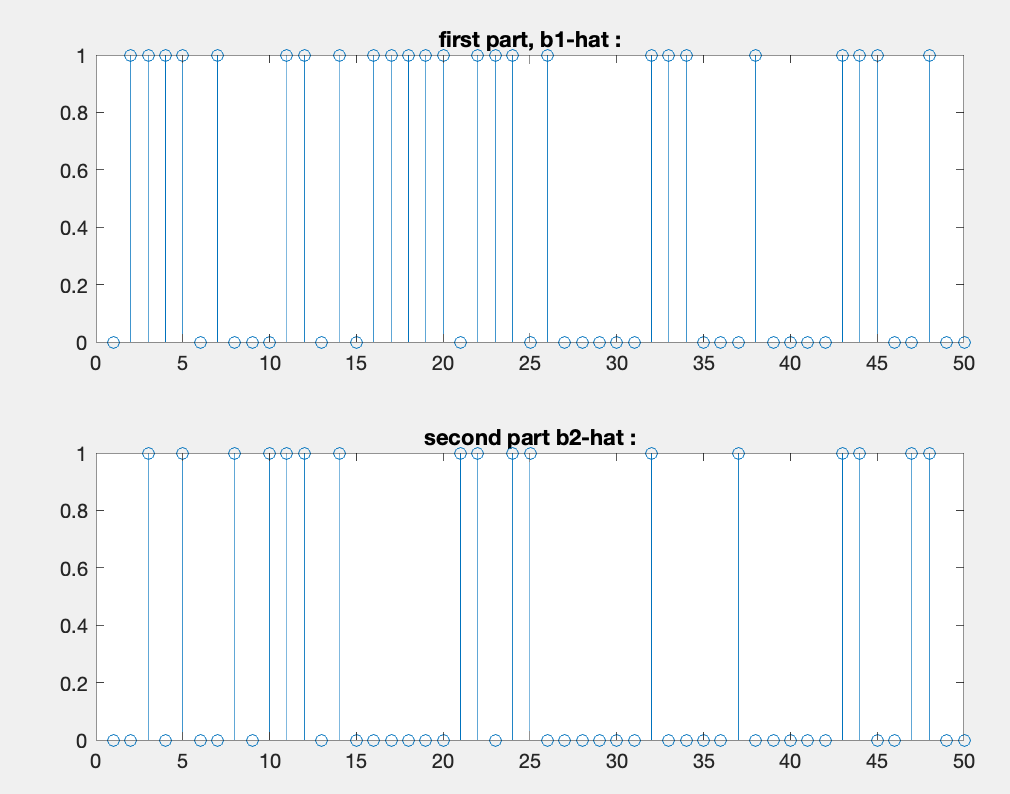
\includegraphics[width=0.5\linewidth]{../img/3.3.7}
		\caption{خروجی دنباله 
			\lr{MatchedFilt}}
		\label{fig:3-3-7}
	\end{figure}
	
	\begin{figure}[h]
		\centering
		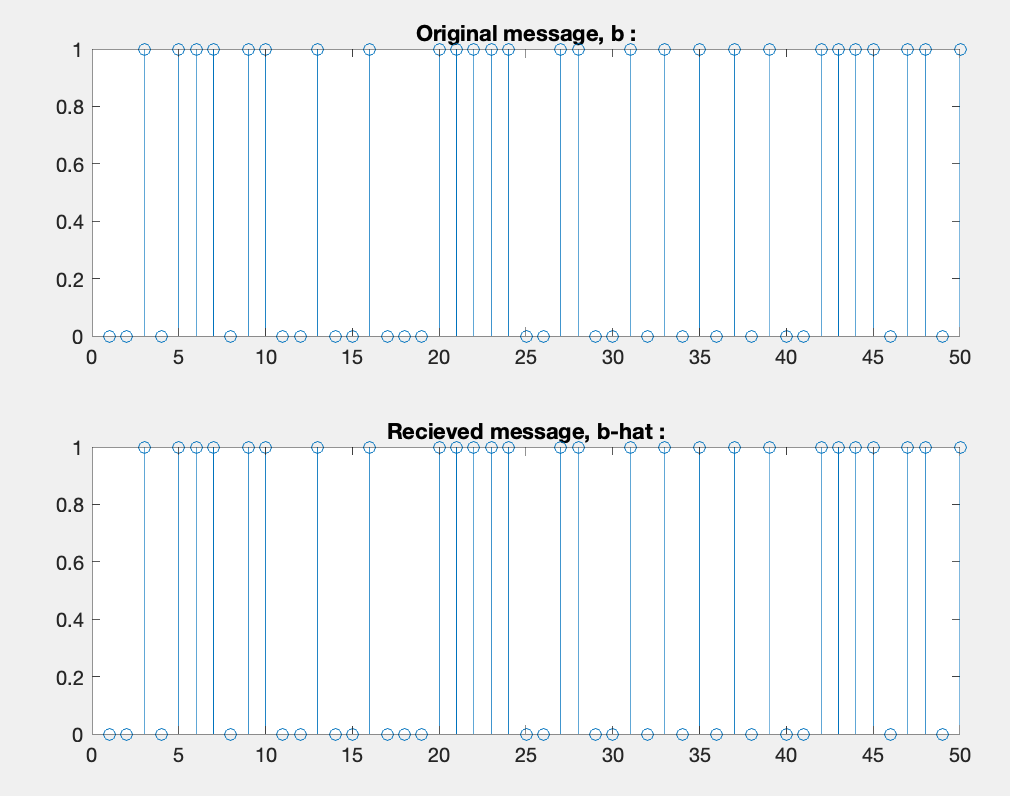
\includegraphics[width=0.7\linewidth]{../img/3.3.8}
		\caption{پیام دریافتی و فرستاده شده}
		\label{fig:3-3-8}
	\end{figure}
	
	
	
	\newpage
	\subsubsection{\lr{AWGN for FSK} }
	در این بخش واریانس خطا را افزایش میدهیم و میزان احتمال خطا نموداری مانند زیر خواهد داشت.
	همچنین همانطور که میبینید نمودار به شدت تیز است و نشان میدهد برای واریانس نویز یکسان این حالت از مابقی حالات به شدت اسیب پذیر تر است و خطای بیشتری دارد.
	\begin{figure}[H]
		\centering
		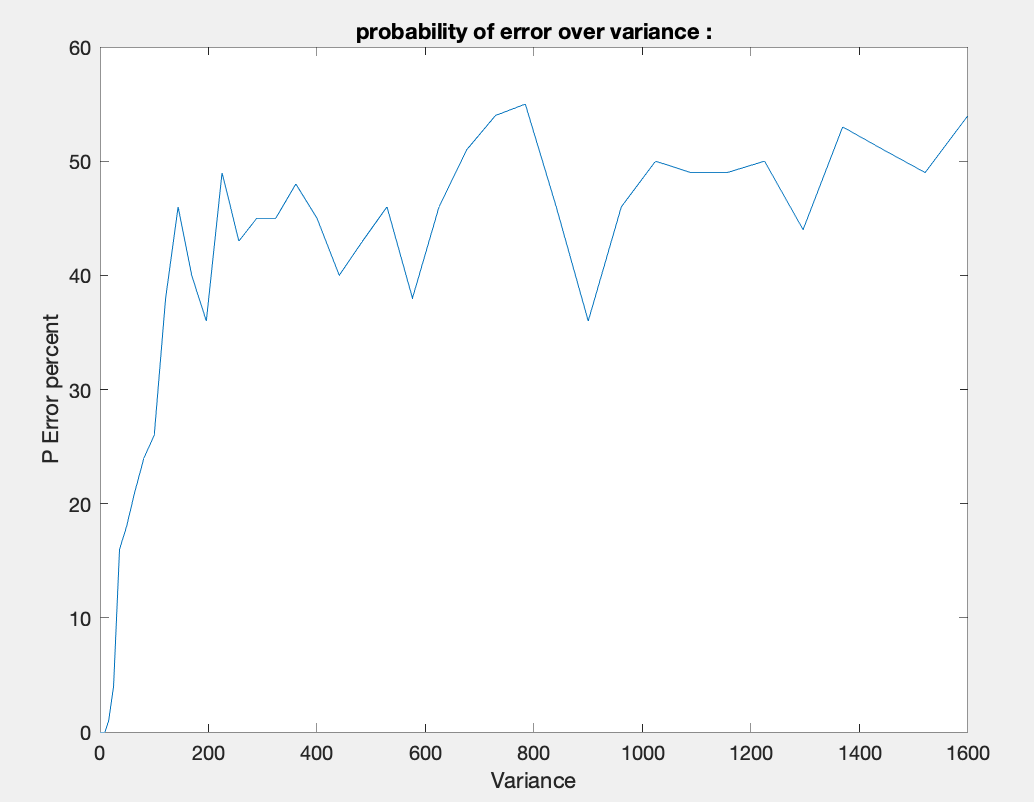
\includegraphics[width=0.6\linewidth]{../img/3.3.10}
		\caption{نمودار خطا بر حسب واریانس نویز}
		\label{fig:3-3-10}
	\end{figure}
	
	\newpage
	همچنین نمودار در بازه بزرگ تر مانند زیر است که به احتمال پنجاه درصد میل میکند که به دلیل کاملا رندوم شدن خروجی با توجه به نویز زیاد است.
	\begin{figure}[H]
		\centering
		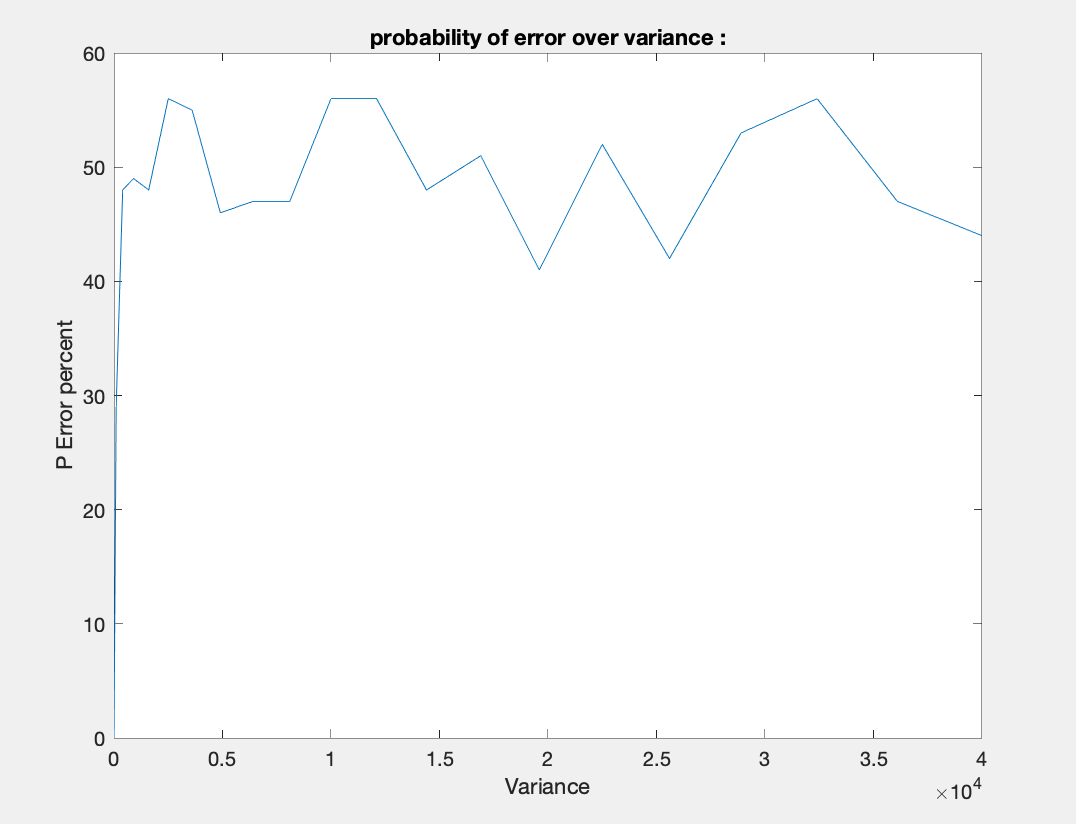
\includegraphics[width=0.6\linewidth]{../img/3.3.9}
		\caption{نمودار خطا بر حسب واریانس نویز در بازه بزرگ تر}
		\label{fig:3-3-9}
	\end{figure}
	
	\newpage
	\subsubsection{\lr{Scatter Plot}}
	در این بخش نمودار منظومه سیگنال به ازای شش واریانس مختلف مانند زیر رسم شده است که هر چه واریانس افزایش میابد فشردگی نقاط حول نقاط اصلی کم تر و کم تر میشود.
	\begin{figure}[H]
		\centering
		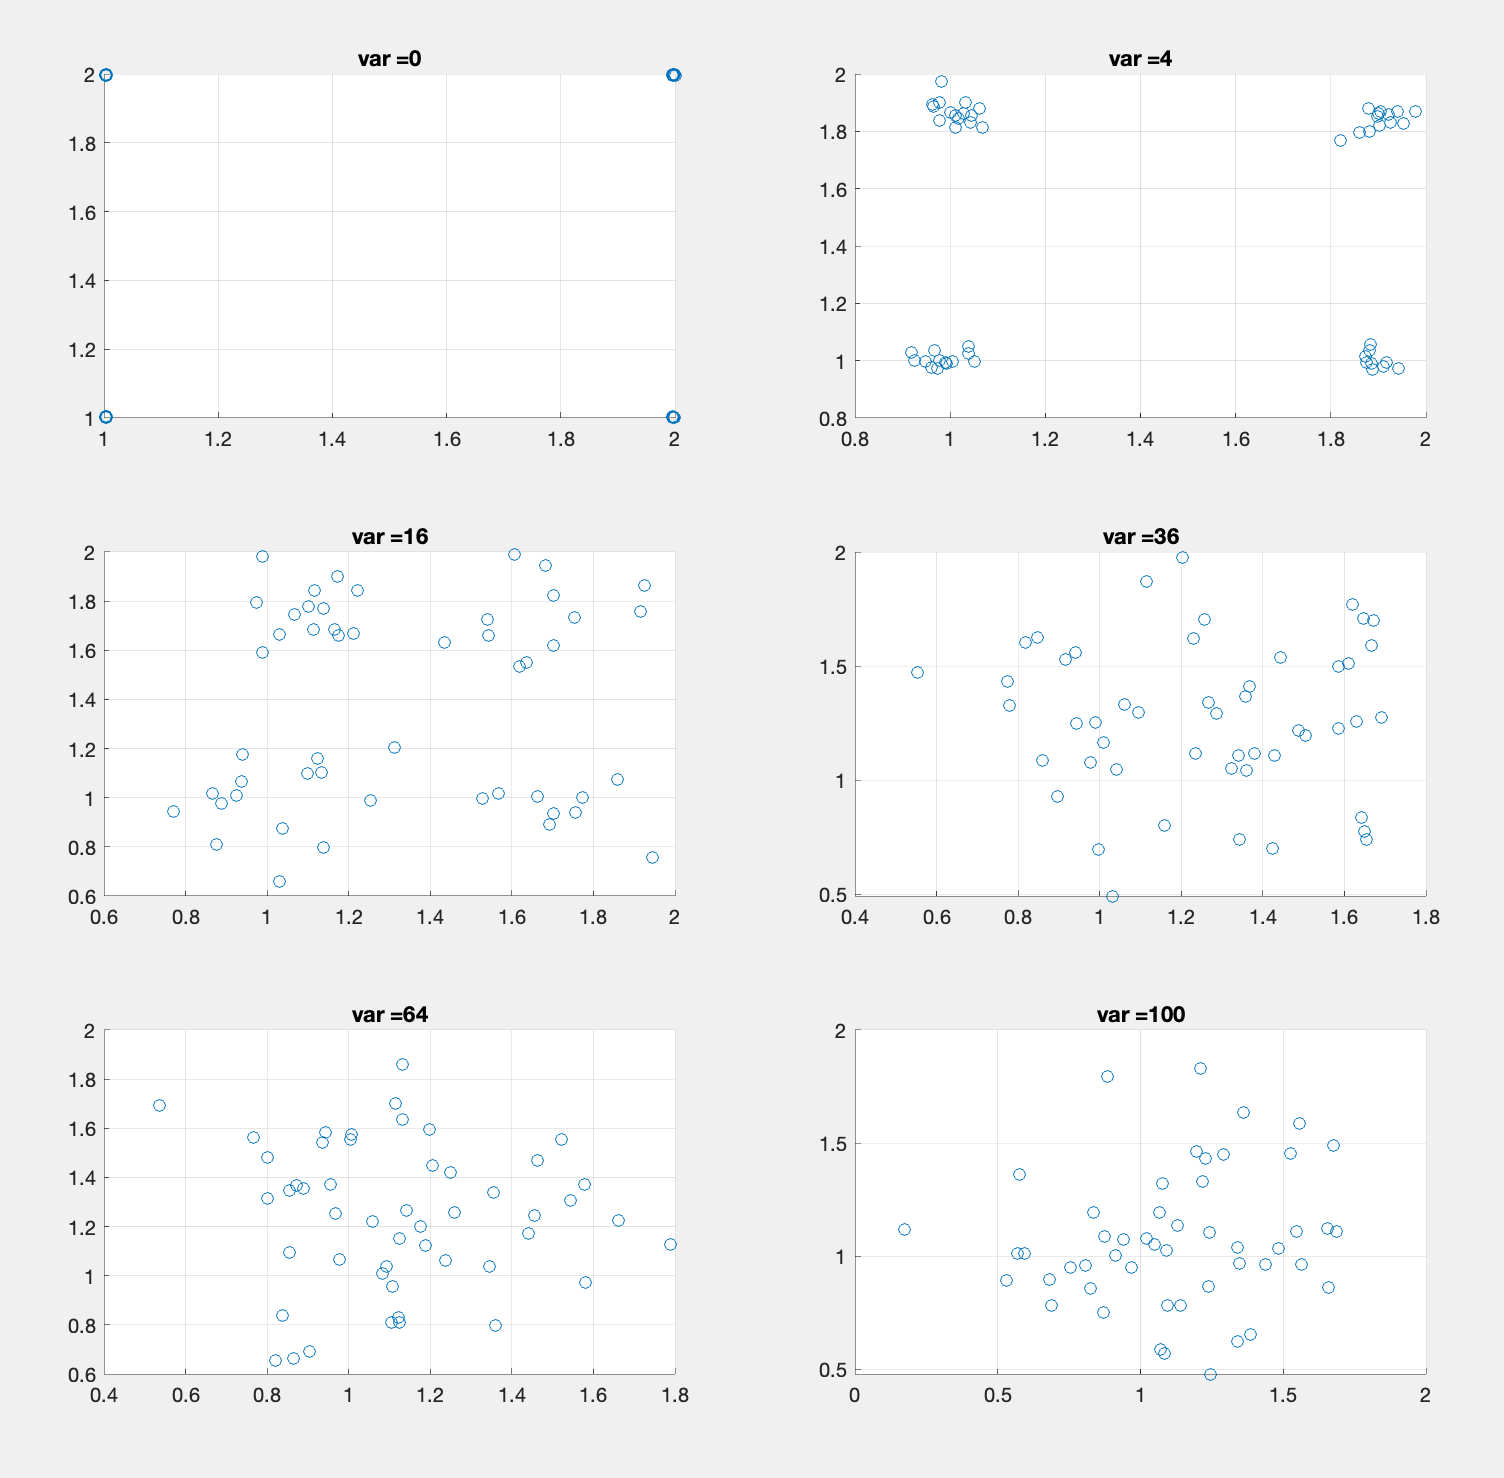
\includegraphics[width=0.8\linewidth]{../img/3.3.11}
		\caption{منظومه سیگنالی}
		\label{fig:3-3-11}
	\end{figure}

	\subsection{برسی این سه حالت}
	همانطور که دیدید در حالت اخر با توجه به پهنای باند کانال کمی مشکل در دریافت صفر و یک داریم و خطا بسیار بیشتر و شدید تر نسبت به دو حالت قبلی است و ماژولیشن اول از همگی ساده تر و دقیق تر است.
	
	\newpage
	\section{انتقال دنباله ای از اعداد ۸ بیتی}
	کد این بخش در 
	\lr{Q4.m}
	قرار دارد.
	
	\subsection{توابع}
	توابع این بخش همانطور که خواسته شده نوشته و تست شده اند و در فولدر 
	\lr{Codes}
	قرار دارد.
	\subsection{AWGN}
	در این بخش نیز سیگنال تبدیل شده به باینری و سپس مخابره شده و نمودار واریانس خروجی بر حسب واریانس نویز رسم شده است.
	\begin{figure}[H]
		\centering
		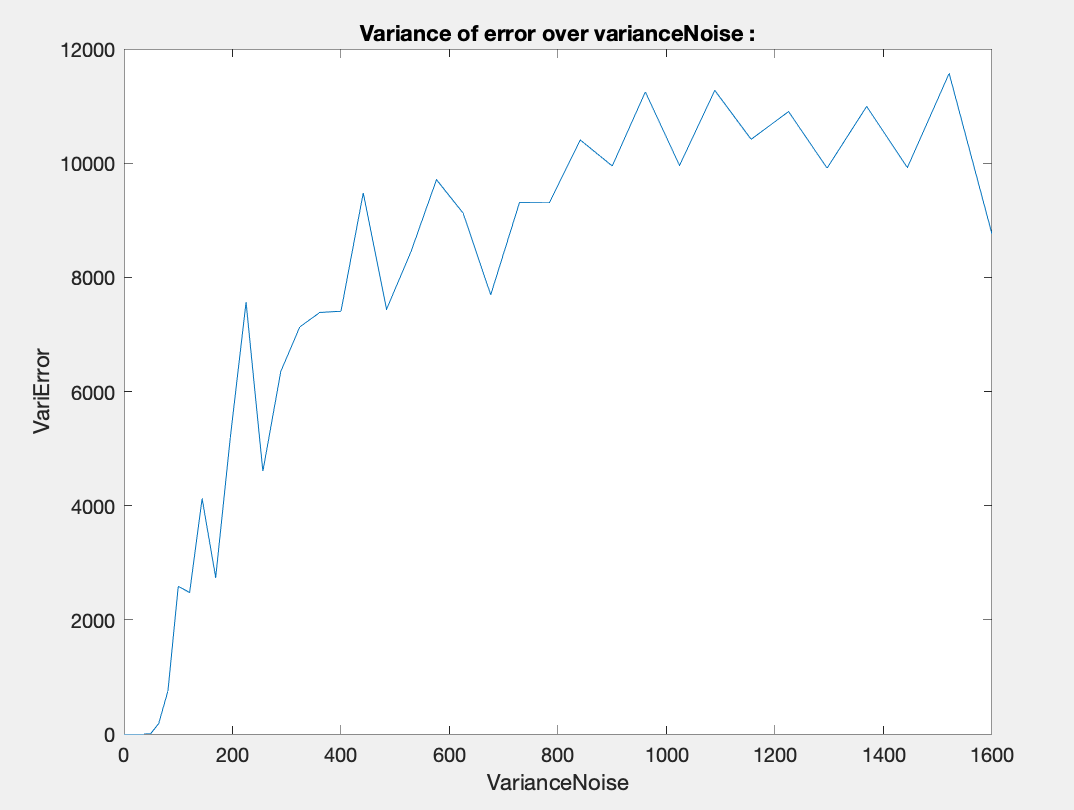
\includegraphics[width=0.8\linewidth]{../img/4.2.1}
		\caption{واریانس خطا بر حسب نویز}
		\label{fig:4-2-1}
	\end{figure}
	
	\newpage
	همچنین نمودار با بازه بیشتر برای بخش اخر :
	\begin{figure}[H]
		\centering
		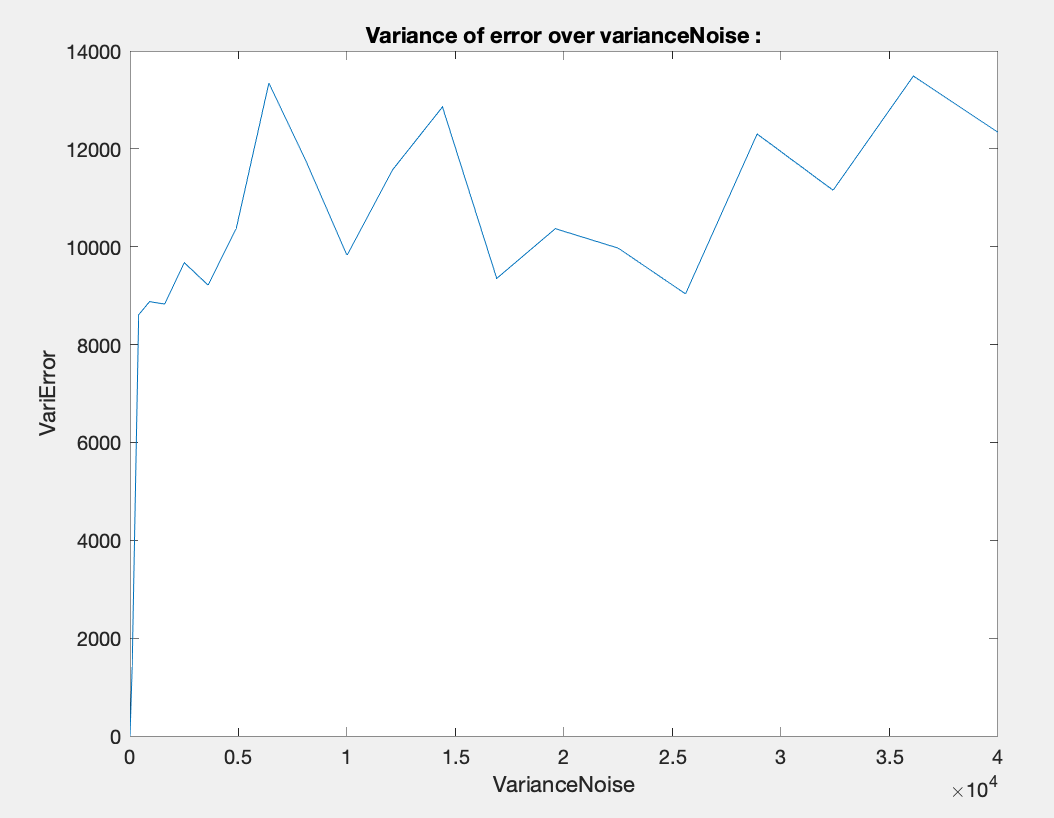
\includegraphics[width=0.8\linewidth]{../img/4.2.2}
		\caption{واریانس خطا بر حسب نویز}
		\label{fig:4-2-2}
	\end{figure}

	\newpage
	\subsection{\lr{histogram}}
	توزیع خطا به ازای واریانس های زیر رسم شده است. که در واریانس نویز کم با احتمال یک بی خطاست و با افزایش نویز به سمت توضیع مثلثی میرود.
	\begin{figure}[H]
		\centering
		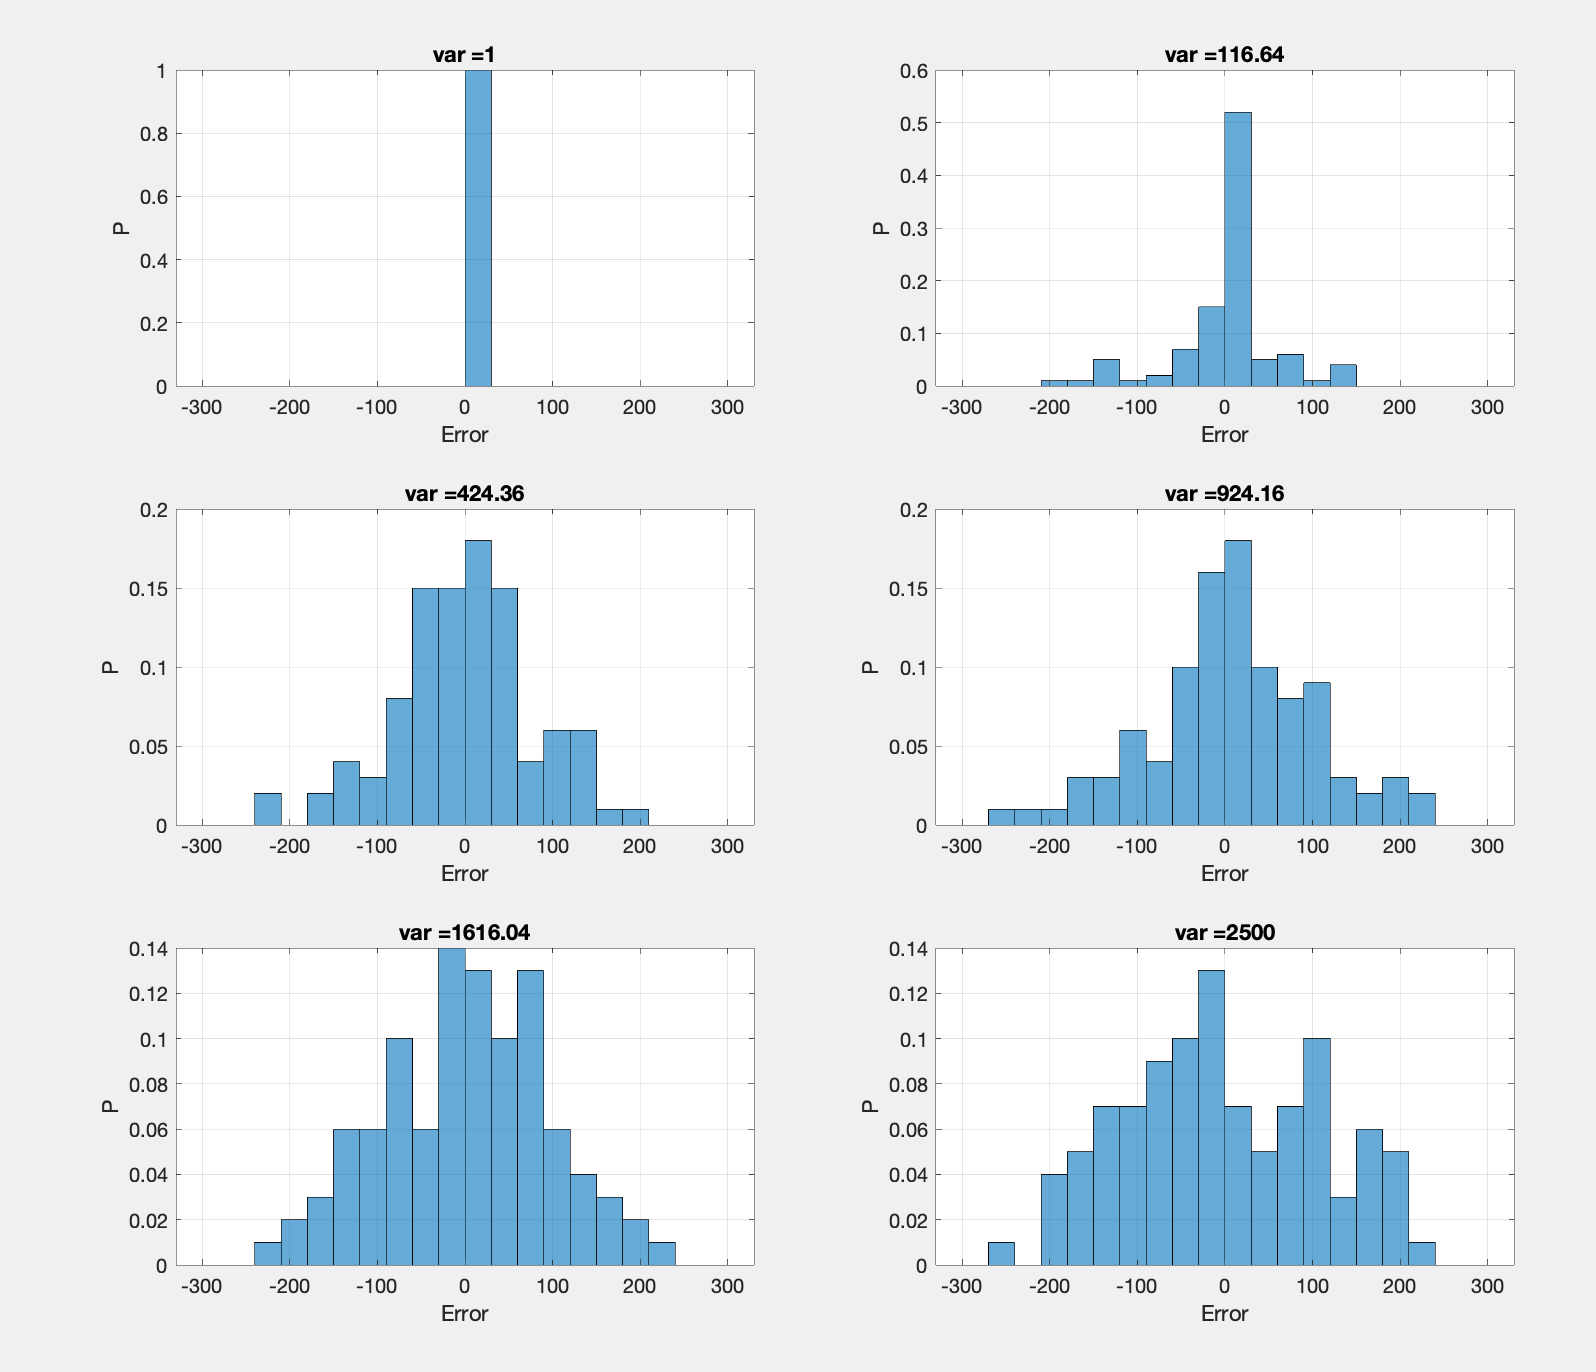
\includegraphics[width=0.8\linewidth]{../img/4.3}
		\caption{واریانس خطا بر حسب نویز}
		\label{fig:4-3}
	\end{figure}
	
	\newpage
	\subsection{روش تحلیلی}
	 که محاسبات مانند تصویر زیر است که عدد نهایی به مقدار به دست امده در بخش دوم بسیار نزدیک است.
	 \lr{$10923.5 = 12000$}
	 
	 \begin{figure}[H]
	 	\centering
	 	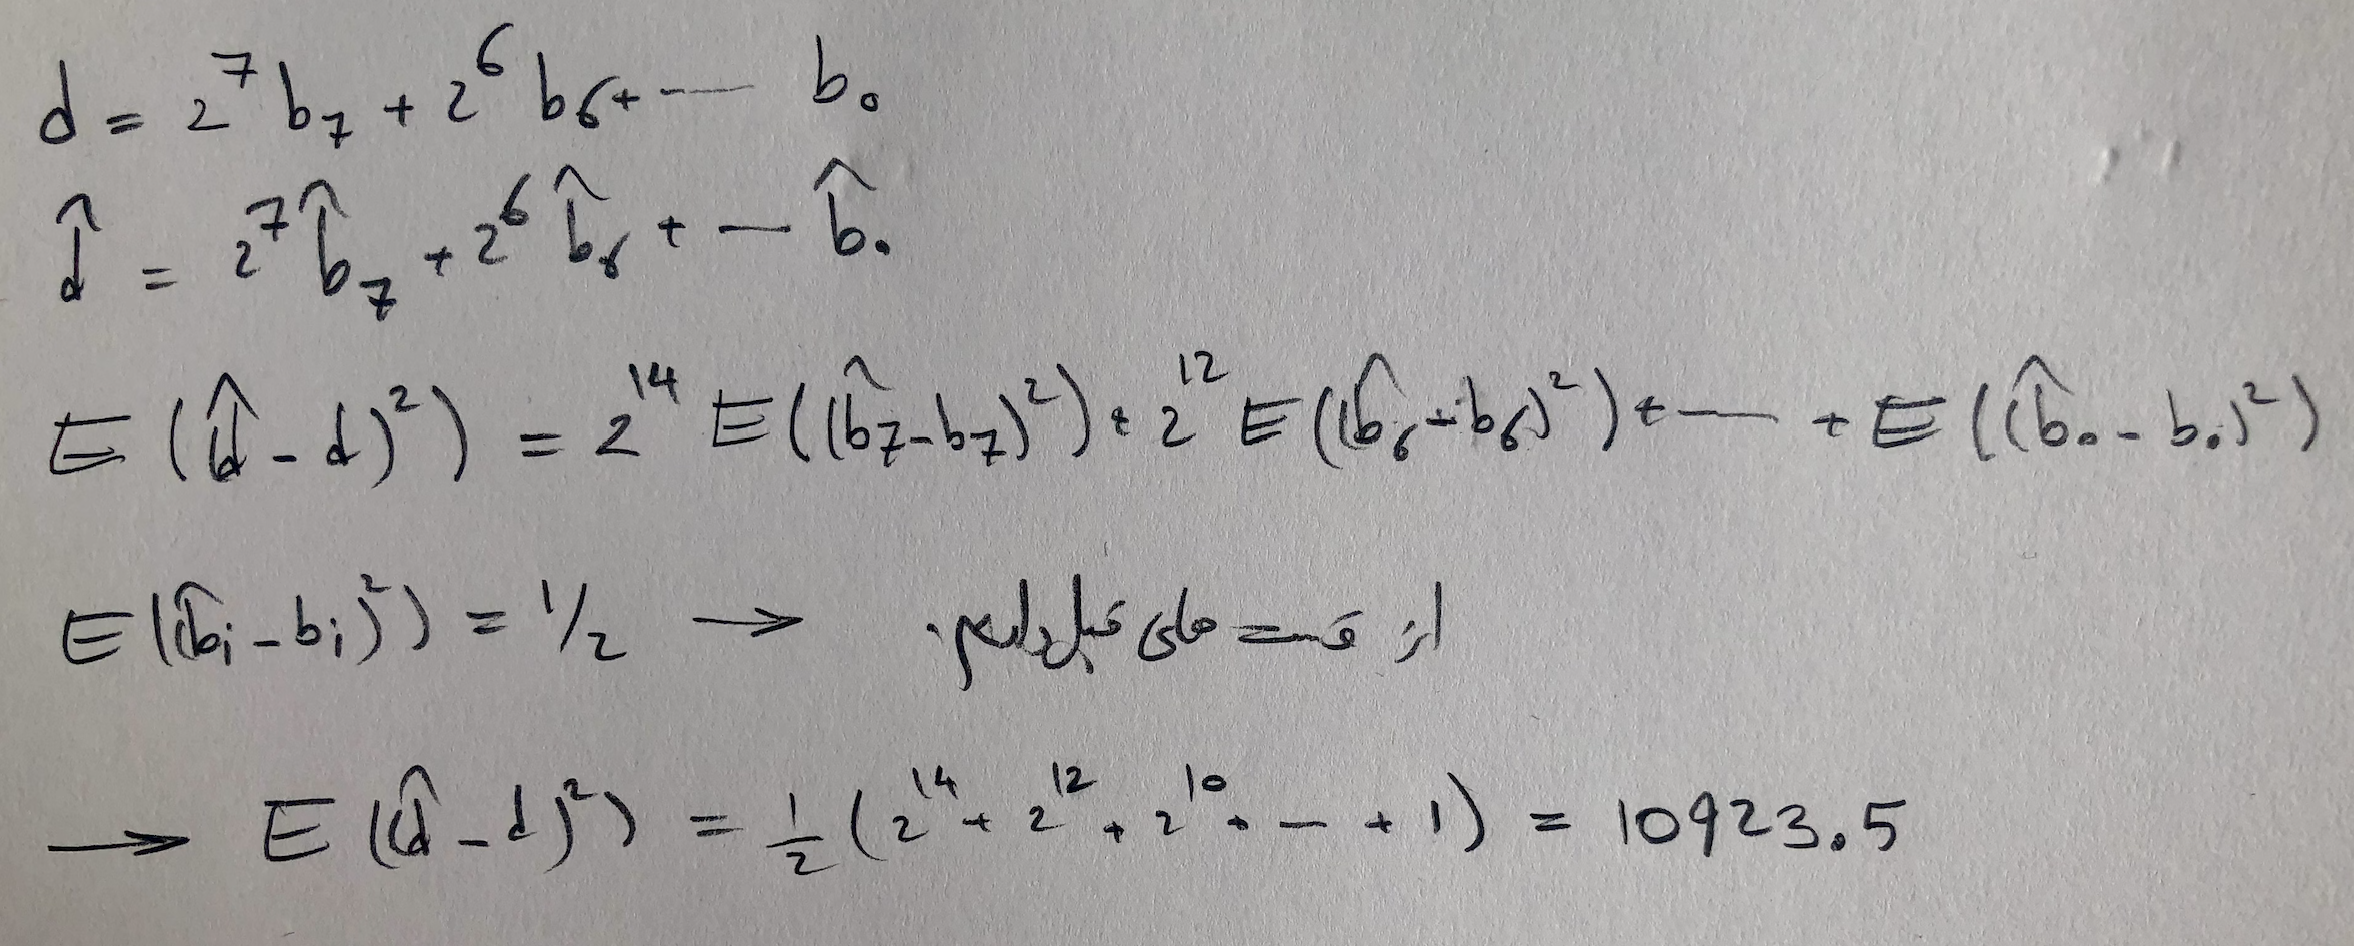
\includegraphics[width=0.9\linewidth]{../img/4.4}
	 	\caption{روش تحلیلی}
	 	\label{fig:4-4}
	 \end{figure}	
	 	
	 \newpage	
	 \section{کدینگ منبع}
	 \subsection{برسی کد ها}
	 \par
	ا) مشکل کد 
	 \lr{C1}
	 این است که برای هر دو حرف بی و دی از کد ۱۰ استفاده شده و در گیرنده نمیتوان این دو حرف را از هم تفکیک کرد.
	 
	 \par
	 \noindent
	 ب) مشکل کد 
	 \lr{C2}
	نیز این است که حرف 
	 \lr{d}
	 با رشته 
	 \lr{ab}
	 قابل تفکیک نیست.
	 \par
	 \noindent
	 ج) همانطور که در متن امده است اگر یک صفر بگیریم نمیتوانیم بلافاصله بگوییم که حرف 
	 \lr{a}
	 را گرفتیم و همینطور برای مابقی حروف اگر طول کد 
	 \lr{n}
	 باشد باید به اندازه 
	 \lr{n+1}
	 بیت صبر کنیم و تاخیر داشته باشیم.
	 
	 \subsection{کد های پیشوندی}
	 مسئله بهینه سازی در زیر حل شده و طول کد های منبع بدست امده است.
	 
	 \begin{figure}[H]
	 	\centering
	 	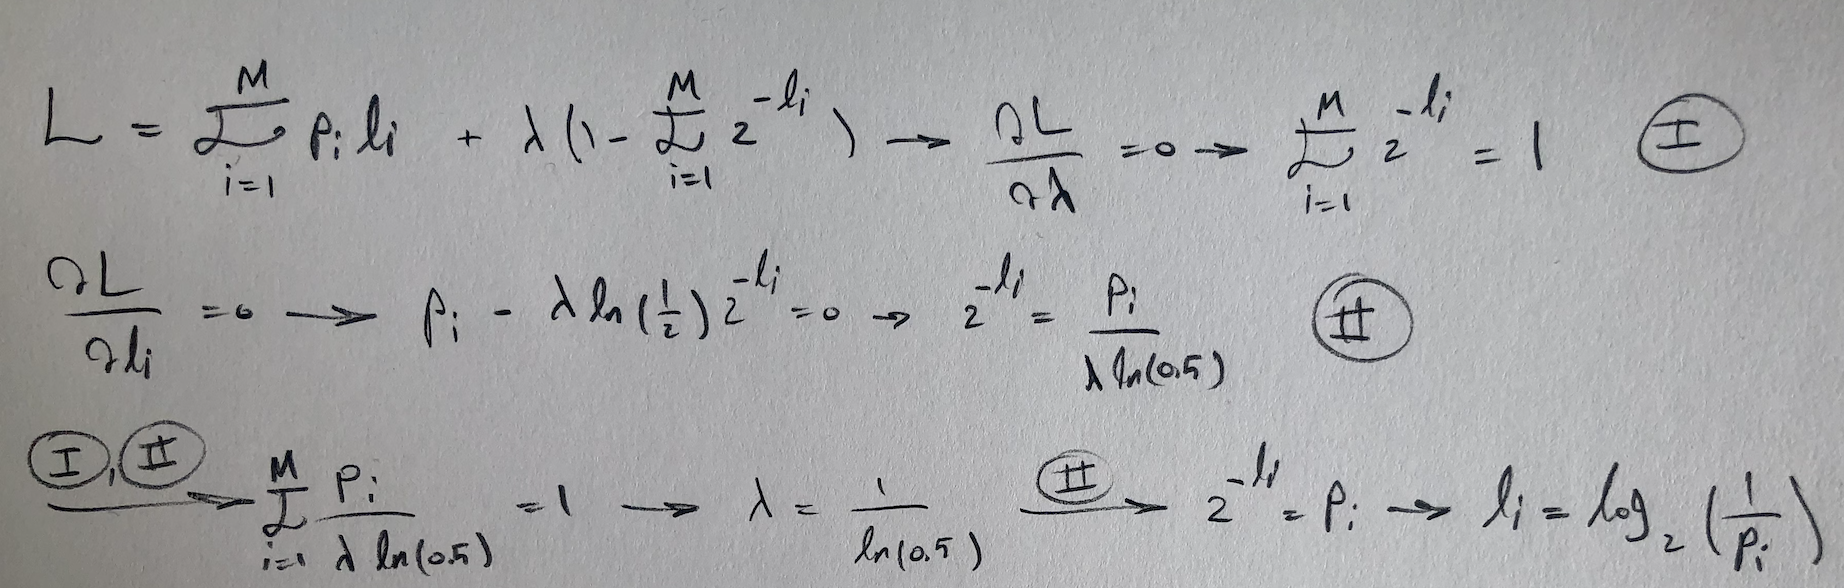
\includegraphics[width=0.9\linewidth]{../img/5.2}
	 	\caption{لاگرانژ طول کد}
	 	\label{fig:5-2}
	 \end{figure}
 
 	\subsection{کلمه کد ها}
 	کلمه کد ها مانند زیر است که یکتا نیست و موارد ساده تر در کد متلب استفاده شده است.
 	 \begin{figure}[H]
 		\centering
 		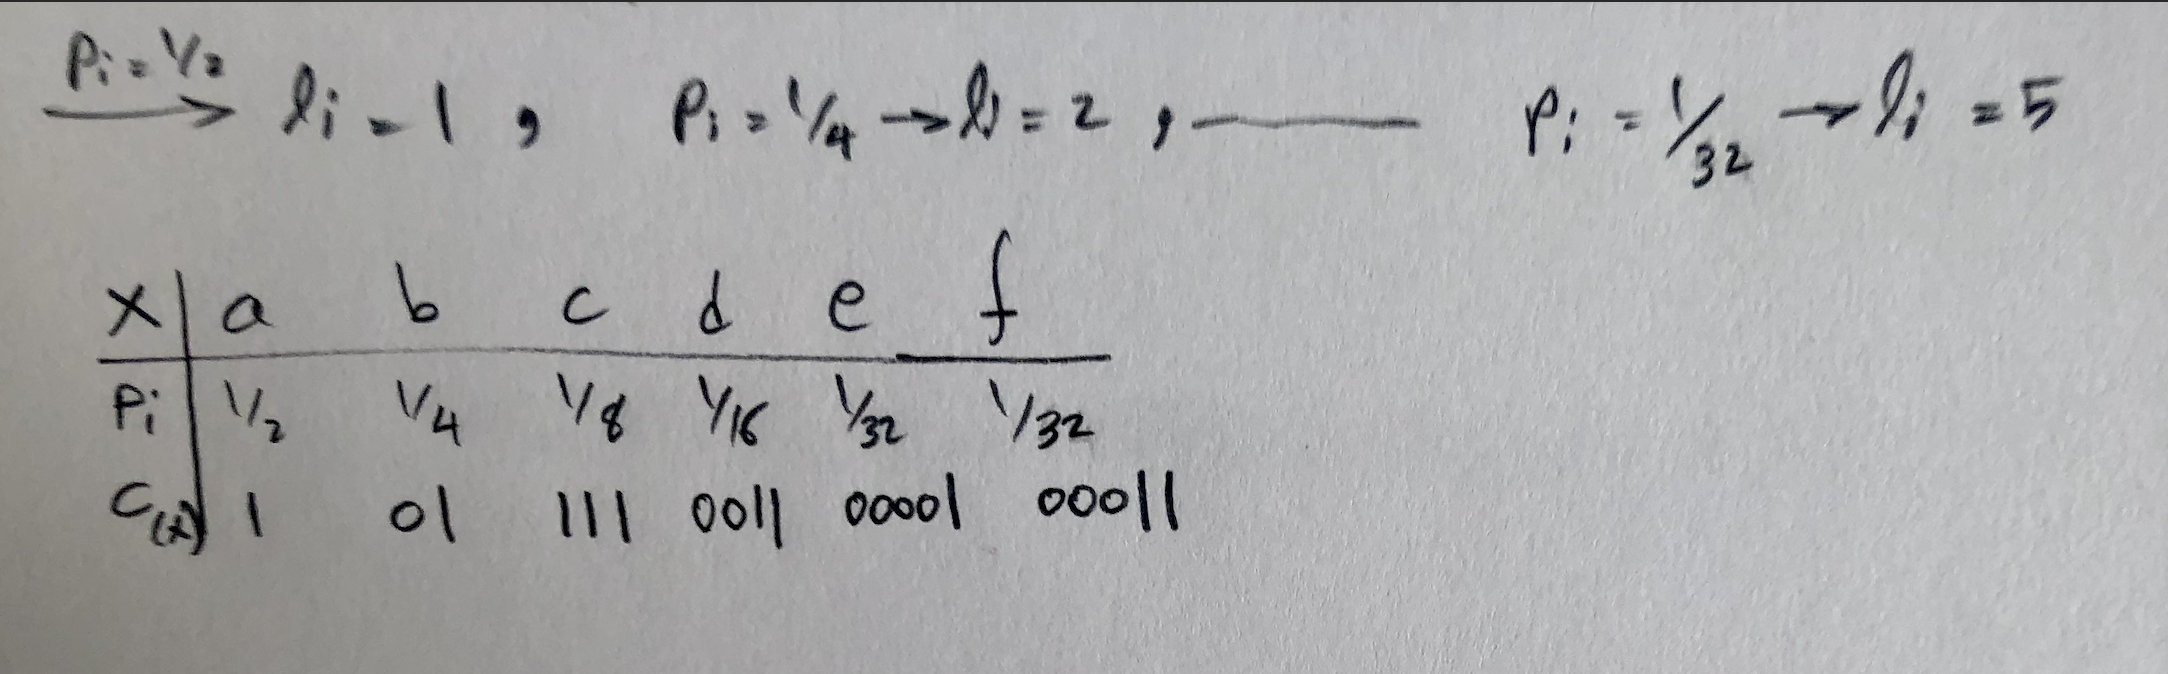
\includegraphics[width=0.9\linewidth]{../img/5.3}
 		\caption{کلمه کد ها}
 		\label{fig:5-3}
 	\end{figure}
 	
 	\subsection{طول متوسط کلمه کد}
 	طول متوسط به سادگی مانند زیر محاسبه شده است.
 	\begin{figure}[H]
 		\centering
 		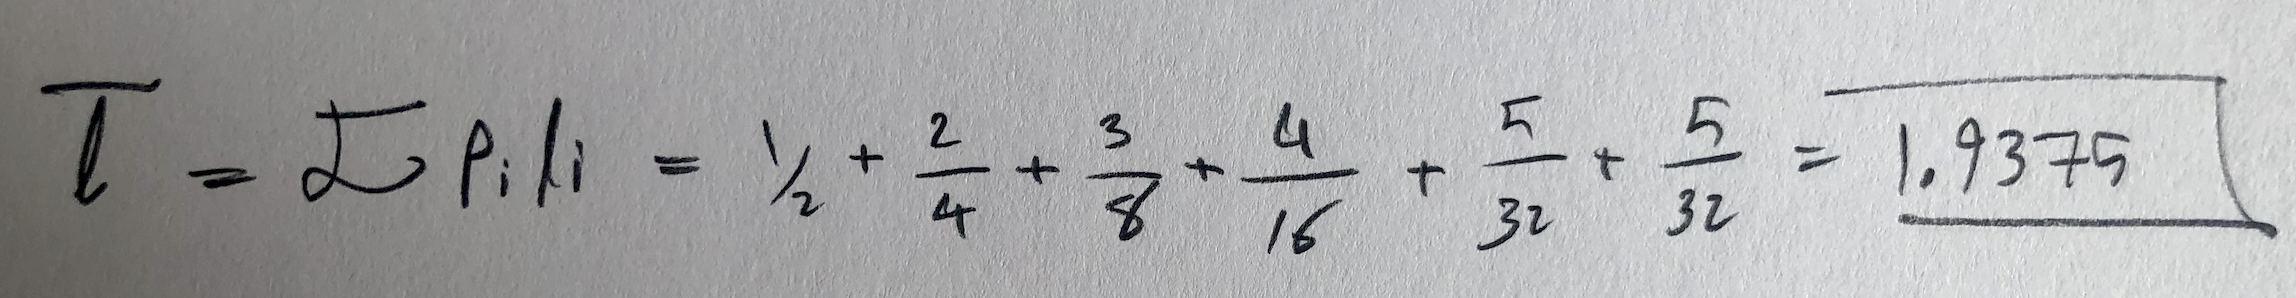
\includegraphics[width=0.9\linewidth]{../img/5.4}
 		\caption{متوسط طول کد}
 		\label{fig:5-4}
 	\end{figure}
 
 
\end{document}